% !TEX encoding = UTF-8 Unicode
\documentclass[12pt,twoside,a4paper]{report}
\setcounter{tocdepth}{2}
\usepackage[]{geometry}
\setlength{\headheight}{15.0pt}
\usepackage[utf8]{inputenc}
\usepackage[T1]{fontenc}
\usepackage[francais]{babel}
\usepackage{graphicx}

% header
\usepackage{fancyhdr}
\pagestyle{fancy}

% code listings
\usepackage{listings}

\usepackage[usenames,dvipsnames,svgnames,table,xcdraw]{xcolor}
\usepackage{pdfpages}

\definecolor{olivegreen}{HTML}{3C8031}

\usepackage[T1]{fontenc}
\usepackage[scaled]{beramono}
\newcommand\Small{\fontsize{9}{9.2}\selectfont}
\newcommand*\LSTfont{\Small\ttfamily\SetTracking{encoding=*}{-60}\lsstyle}

\definecolor{lightgray}{rgb}{.9,.9,.9}
\definecolor{darkgray}{rgb}{.4,.4,.4}
\definecolor{purple}{rgb}{0.65, 0.12, 0.82}
\lstdefinelanguage{JavaScript}{
  keywords={break, case, catch, continue, debugger, default, delete, do, else, false, finally, for, function, if, in, instanceof, new, null, return, switch, this, throw, true, try, typeof, var, void, while, with},
  morecomment=[l]{//},
  morecomment=[s]{/*}{*/},
  morestring=[b]',
  morestring=[b]",
  ndkeywords={class, export, boolean, throw, implements, import, this},
  keywordstyle=\color{blue}\bfseries,
  ndkeywordstyle=\color{darkgray}\bfseries,
  identifierstyle=\color{black},
  commentstyle=\color{purple}\ttfamily,
  stringstyle=\color{red}\ttfamily,
  sensitive=true
}

\lstset{ %
  basicstyle=\footnotesize\ttfamily,        % the size of the fonts that are used for the code
  breakatwhitespace=false,         % sets if automatic breaks should only happen at whitespace
  breaklines=true,                 % sets automatic line breaking
  commentstyle=\color{olivegreen},    % comment style
  escapeinside={\%*}{*)},          % if you want to add LaTeX within your code
  extendedchars=true,              % lets you use non-ASCII characters; for 8-bits encodings only, does not work with UTF-8
  frame=single,	                   % adds a frame around the code
  keepspaces=true,                 % keeps spaces in text, useful for keeping indentation of code (possibly needs columns=flexible)
  keywordstyle=\color{blue},       % keyword style
  lineskip={-1.5pt},
  numbers=left,                    % where to put the line-numbers; possible values are (none, left, right)
  numbersep=5pt,                   % how far the line-numbers are from the code
  numberstyle=\tiny\color{black}, % the style that is used for the line-numbers
  rulecolor=\color{black},         % if not set, the frame-color may be changed on line-breaks within not-black text (e.g. comments (green here))
  showspaces=false,                % show spaces everywhere adding particular underscores; it overrides 'showstringspaces'
  showstringspaces=false,          % underline spaces within strings only
  showtabs=false,                  % show tabs within strings adding particular underscores
  stepnumber=1,                    % the step between two line-numbers. If it's 1, each line will be numbered
  stringstyle=\color{purple},     % string literal style
  tabsize=2,	                   % sets default tabsize to 2 spaces
}

% link
\PassOptionsToPackage{hyphens}{url}\usepackage{hyperref}

% glossary
\usepackage[automake]{glossaries}

\usepackage{bytefield}

\usepackage{amsmath}

\usepackage{subfig}

\usepackage{caption}

\usepackage[section]{placeins}

\usepackage[export]{adjustbox}

\usepackage{wrapfig}

\usepackage{rotating}

\usepackage{longtable}

\usepackage{csquotes}

\newcommand\MyLBrace[2]{%
  \left.\rule{0pt}{#1}\right\}\text{#2}}

\newcommand\MyRBrace[2]{%
  \left.\rule{0pt}{#1}\text{#2}\right\{}


\makeglossaries

\newglossaryentry{open-source}
{
	name=open-source,
	description={qualifie un logiciel dont le code initial est mis à disposition du grand public}
}

\newglossaryentry{DOM}
{
	name={Document Object Model},
	description={est l'arbre d'éléments qui compose un fichier HTML}
}

\newglossaryentry{NLP}
{
	name={Natural Language Processing},
	description={est une catégorie de techniques algorithmiques visant à comprendre un texte écrit dans une langue humaine}
}

\newglossaryentry{LSI}
{
	name={Latent Semantic Indexing},
	description={est le nom d'une catégorie de techniques algorithmiques visant à comprendre les relations entre des documents écrits dans une langue humaine}
}

\newglossaryentry{TF-IDF}
{
	name={Term Frequency-Inverse Document frequency},
	description={est le nom d'une technique de de keyword extraction}
}

\newglossaryentry{RAKE}
{
	name={Rapid Automatic Keyword Extraction},
	description={est le nom d'une technique de de keyword extraction}
}

\newglossaryentry{LDA}
{
	name={Latent Dirichelet Allocation},
	description={est le nom d'un modèle de topic modeling}
}

\newglossaryentry{stopword}
{
	name={stopword},
	description={est le nom donné aux mots qui servent généralement de liaison, que nous cherchons à ignorer lors d'analyses}
}

\newglossaryentry{endpoint}
{
	name={endpoint},
	description={est le nom donné à un point autonome accessible d'une API}
}

\newglossaryentry{API}
{
	name={Application Programming Interface},
	description={est un ensemble de méthodes invocables permettant l'accès à des fonctionnalités d'un logiciel}
}

\begin{document}


\includepdf[pages={1}]{images/garde.pdf}

\def\myTitle{Développement d'une Application Web pour la Visualisation et la Recherche de Données Médicales}
\def\myName{Kewin Dousse}
\def\myUni{HES-SO}
\def\myDepartment{TIC}
\def\mySupervisors{Sandy Ingram}
\def\myExpert{?}


\begin{abstract}

Le but de ce projet est de concevoir et développer une application Web multi-plateforme pour la recherche et la visualisation de données médicales.

\smallskip
\noindent \textbf{Keywords.} Web, Visualisation

\end{abstract}
\setcounter{page}{3}
\hypersetup{pageanchor=true}

\tableofcontents
\listoffigures

\chapter{Introduction}
\section{Contexte}

	En janvier 2014, l'ONG Internet Society a publié le document Digital footprints qui aborde la question de la capacité que les webtrackers ont de définir le profile personnel des usagers d'Internet. [1]
	En 2016, Michal Kosinski chercheur à Stanford révèle les possibilités de définir un profile précis simplement en analysant les préférences (likes) enregistrées dans un profile Facebook. L'étude révèle que ce type d'analyse permet de mieux connaître une personne que ses proches et même de prévoir de probables comportements avec une grande précision. De plus, lors d'événements politiques majeurs ces techniques de profiling auraient été utilisées, comme dans le cadre des campagnes pour le Brexit ou pour l'élection du président américain Trump. [2]

	Bla contexte \gls{mot}.

	Bla liste
	\begin{enumerate}
		\item Truc 1
		\item Truc 2
	\end{enumerate}

\section{Objectifs}

	Le but de ce projet est de concevoir et d'implémenter un outil d'analyse de comportement d'utilisateurs d?applications Web pour révéler les potentiels de détection de profile des personnes (préférences, centre d'intérêt, orientations et opinions) en analysant les interactions et les informations échangées avec les applications Web. L'application développée dans ce projet a pour le but de sensibiliser le public et les médias à la question du profiling sur internet.

	Bla liste
	\begin{itemize}
		\item Truc 1
		\item Truc 2
	\end{itemize}

\section{Contraintes}

	Bla liste
	\begin{itemize}
		\item Truc 1
		\item Truc 2
	\end{itemize}

\section{Méthodologie}

	Bla
\chapter{Analyse}
%%%%%%%%%%%%%%%%%%%%%%%%%
%                          %
% ----- INTRODUCTION ----- %
%                          %
%%%%%%%%%%%%%%%%%%%%%%%%%%

\section{Projet similaire}

	\subsection{Introduction}

		Afin de placer notre recherche dans les connaissances actuelles, nous nous intéressons d'abord aux recherches récentes partageant un objectif semblable au nôtre.

		Michal Kosinski se présente sur son site web\cite{michal-kosinski} comme un "psychologist and data scientist". L'étude qu'il a co-rédigée à l'Université de Stanford en 2016 a eu un impact important sur le monde académique et même industriel, en montrant les possibilités techniques ouvertes par la récolte de données simples d'utilisateurs : les "likes" Facebook.

		Il est montré qu'avec un peu plus de 300 "likes" tirés une personne, il est possible de définir avec une précision remarquable (mieux que son époux/épouse) des traits psychologiques, ainsi que d'autres caractéristiques personnelles.

	\subsection{Résumé}

		Une enquête a été menée auprès d'une population variée de personnes possédant un compte Facebook. Les données concernant leurs "likes" ont été récoltées, ainsi que des données personnelles pouvant être disponible (ou non) selon le souhait de l'utilisateur sur Facebook, comme ses informations démographiques. Des tests psychologiques ont été également réalisés par une certaine partie des utilisateurs afin de pouvoir trouver des corrélations entre les pages likées et certains traits psychologiques.

		Cette enquête a rencontré un succès très large, et le nombre de personne ayant répondu à l'enquête, au moins en partie, se compte en millions.

		Les résultats présentés à la fin de l'étude sont inattendus : Michal annonce qu'il est possible de prédire certains comportements d'une personne mieux que son entourage le plus proche.

		Un des modèles crées avec les données récoltées, permet d'estimer le profil psychologique d'un participant selon cinq axes différents, en se basant sur ses likes Facebook. La figure~\ref{a-talk1} montre la précision obtenue par le modèle en fonction du nombre de likes utilisé en entrée.

		\begin{figure}[ht]
			\centering
			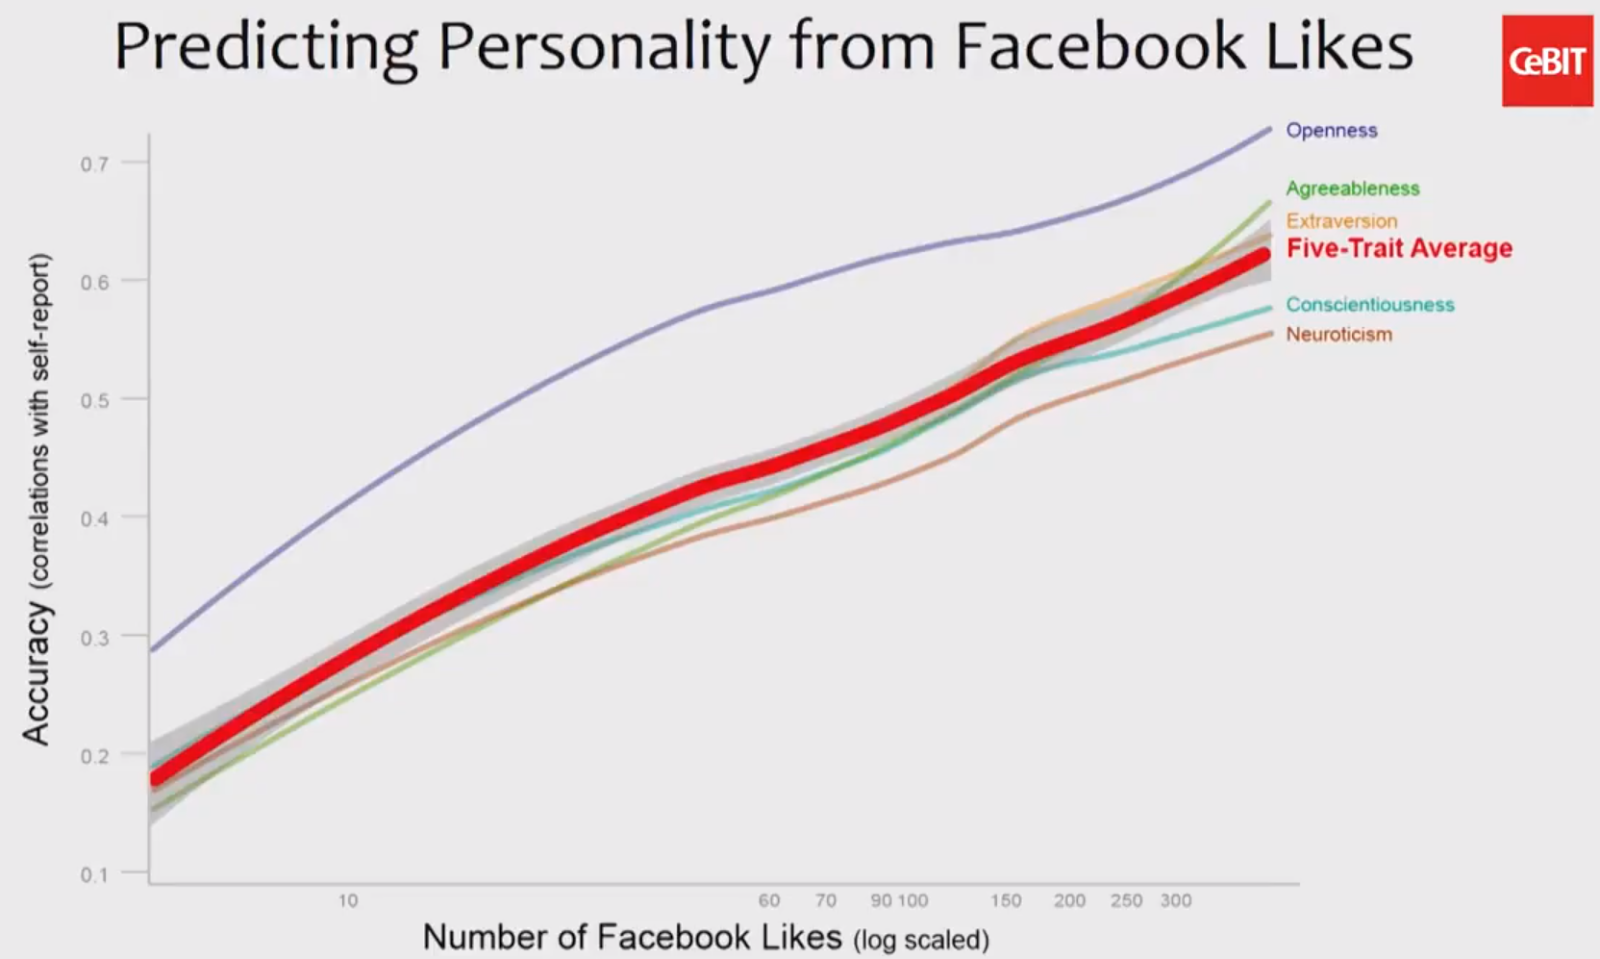
\includegraphics[width=1\textwidth]{images/analysis/talk1}
			\caption{Précision moyenne du modèle prédisant la personnalité d'un utilisateur en fonction du nombre de likes analysés\cite{kosinski-talk}.}
			\label{a-talk1}
		\end{figure}

		On remarque que la précision de la prédiction de tous les critères augmente avec le nombre de likes utilisés, ce qui n'est pas surprenant. En revanche, le tableau~\ref{a-talk-table1} montre le lien entre le nombre de likes utilisés et la précision moyenne atteinte par l'algorithme, et compare ces valeurs à la précision atteinte par d'autres êtres humains.

		\begin{table}[]
			\centering
			\begin{tabular}{lll}
				         & Précision & Nombre de likes \\
				Collègue & 0.27      & 10                            \\
				Ami      & 0.44      & 80                            \\
				Famille  & 0.5       & 100                           \\
				Epoux/se & 0.58      & 250                          
			\end{tabular}
			\caption{Précision atteinte par type de relation avec une personne, et nombre de likes nécessaires au modèle pour égaler sa précision}
			\label{a-talk-table1}
		\end{table}

		On peut voir que la précision de la prédiction de l'algorithme surpasse celle même l'époux/se d'une personne avec 250 likes, ce qui se trouve être légèrement au-dessus du nombre de likes moyen par personne, qui est de 227.

		Les possibilités de prédiction du modèle ne se limitent pas à une simple personne, et les possibilités sont nombreuses. Par exemple, Michal montre qu'il est possible de montrer une corrélation entre les visiteurs d'un certain site web, et une tendance vers certains traits psychologiques. La figure~\ref{a-talk2} montre la personnalité moyenne estimée des visiteurs du site web ```deviantart.com''' par rapport à la moyenne de tous les utilisateurs.

		\begin{figure}[ht]
			\centering
			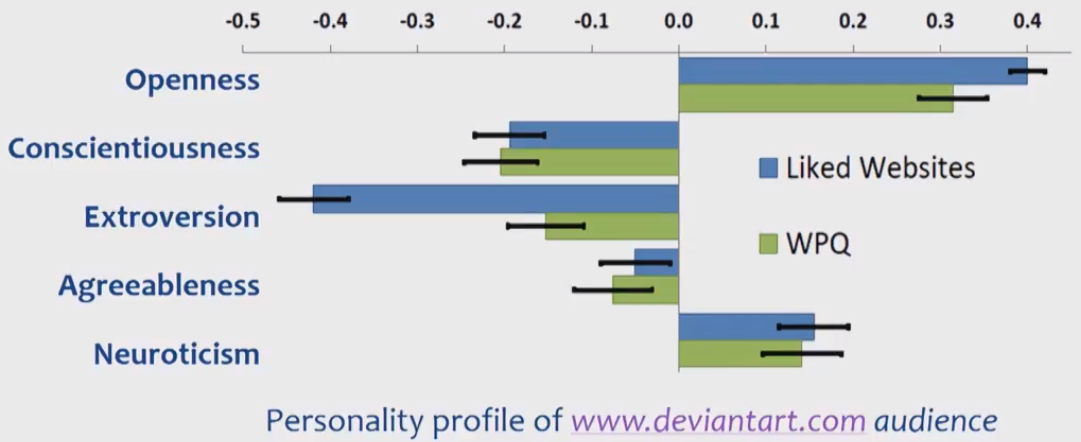
\includegraphics[width=1\textwidth]{images/analysis/talk2}
			\caption{Déviation de la personnalité moyenne estimée d'un visiteur régulier du site ```deviantart.com''' selon les cinq axes psychologiques employés\cite{kosinski-talk}.}
			\label{a-talk2}
		\end{figure}

		Ces corrélations ne sont que quelques exemples parmi un très large éventail de possibles corrélations que le modèle est capable de mettre en lumière. Les implications de telles découvertes sont massives : Il serait par exemple possible de déterminer si un utilisateur sera réceptif ou non à un certain type de publicité, par exemple. Ce genre de problématique touche à plusieurs domaines et n'est pas exactement de notre ressort ici : Des principes éthiques sont en jeu, et le sujet devient de plus en plus délicat. Mais une chose est certaine : Des likes Facebook peuvent révéler énormément d'informations.

	\subsection{Données}

		La quantité de données amassée par l'étude est massive. Non seulement en quantité d'utilisateurs, mais également en diversité de données. Michal Kosinski a mis en place le site web "myPersonnality Project"\cite{mypersonnality} permettant de partager cette source de données avec d'autres chercheurs. Les données comprennent, entre autres :

		\begin{itemize}
			\item Scores de personnalité selon la méthode BIG5 de >3 millions de personnes
			\item Données démographiques de >4 millions de personnes
			\item Localisation géographique de >1.5 million de personnes
			\item Vues politiques de >500'000 personnes
			\item Likes Facebook de >19 millions de personnes
		\end{itemize}

		Le type de données présenté ici n'est qu'un sous-ensemble restreint de l'ensemble des tables présentées, bien qu'il s'agisse ici des données comprenant le plus d'entrées au total.

	\subsection{Acquisition}

		Bien que l'objectif du site web soit de partager l'accès à cette énorme base de données, l'accès à celle-ci est loin d'être aisé. Tout d'abord, Kosinski ne met ces données à disposition que de milieux académiques, il interdit l'utilisation de ces données à des fins commerciales.

		Cependant l'accès n'est pas donné pour autant : Une demande d'accès est à lui envoyer, comprenant une présentation du projet et de ses buts par le biais d'un mail ainsi que le remplissage et l'enregistrement du projet de recherche sur des sites spécialisés.

		Cette étape ne semblait constituer qu'une marche nécessitant un temps restreint, mais un prérequis à l'envoi d'une demande d'accès à la base de données est l'approbation de l'"IRB" (Institutional Review Board), ce qui correspond à un comité d'éthique.

	\subsection{Conclusion}

		Etant donné les délais estimés de l'envoi de la demande à un comité d'éthique responsable puis de la demande d'accès aux données à Kosinski, nous avons écarté cette source de données de la liste principale du projet car nous n'avions pas l'assurance de disposer des données à temps pour la suite de l'étude. Bien qu'il s'agisse certainement d'un ajout conséquent aux données amassées par le projet, nous ne pouvons pas nous permettre de mettre en péril tout l'agenda du projet sur cette source de données.

		Bien que cette base de connaissance ait pu être utile, notre étude va changer de direction. Nous décidons de baser la recherche sur des données que nous récupérerons nous-même.

\section{Outils de tracking}

	\subsection{Trackers}

		Un tracker est un serveur contacté lors du chargement d'une page web par un utilisateur. De nos jours, les pages web sont souvent constituées de contenu provenant de plusieurs serveurs ou domaines différents. Il n'est pas rare qu'une seule page web fasse appel à plus d'une dizaine de domaines différents pour charger une seule page. La figure~\ref{a-nbdomains} montre l'évolution du nombre moyen de domaines contactés pour le chargement d'une seule page web, sur les 1'000 sites web les plus visités mondialement.

		\begin{figure}[h]
			\centering
			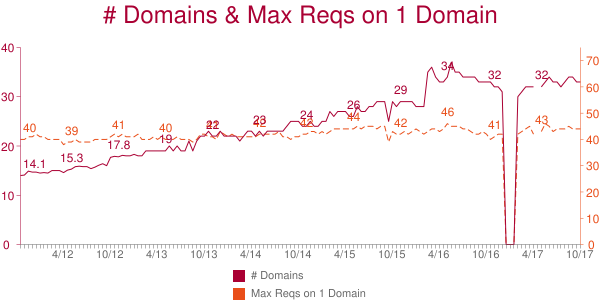
\includegraphics[width=1\textwidth]{images/analysis/nbdomains}
			\caption{Nombre moyen de domaines contactés au chargement d'une page web\cite{nbdomains}.}
			\label{a-nbdomains}
		\end{figure}

		Bien qu'une partie des domaines soient nécessaires à contacter afin de charger du contenu indispensable à la page, une partie d'entre eux ne sert également qu'à des fins statistiques ou publicitaires. Par exemple, ceux-ci peuvent récupérer des informations sur l'utilisateur et son navigateur afin de lui proposer des publicités ciblées sur ses intérêts. Cette pratique est aujourd'hui courante, comme le montre la prochaine sous-section.

	\subsection{Marché}

		Etant donné que nous nous intéressons aux données des utilisateurs récupérées lors de la navigation Web, nous cherchons à connaître quels sont les plus grand trackers sur le web.

		La figure~\ref{analytics-usage} montre la part de marché qu'occupe Google Analytics ainsi que ses compétiteurs sur les sites web Suisses.

		\begin{figure}[!h]
			\centering
			\subfloat[Utilisation de services d'analyse et de tracking\label{a-analytics-usage1}]{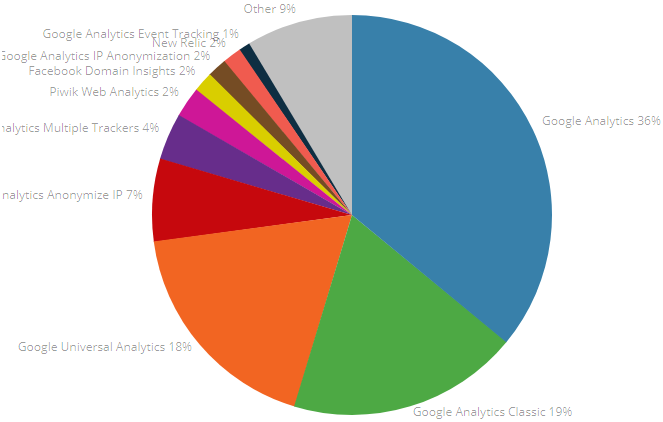
\includegraphics[width=0.45\textwidth,valign=t]{images/analysis/analytics-usage1}}
			\subfloat[Utilisation de services de mesure d'audience\label{a-analytics-usage2}]{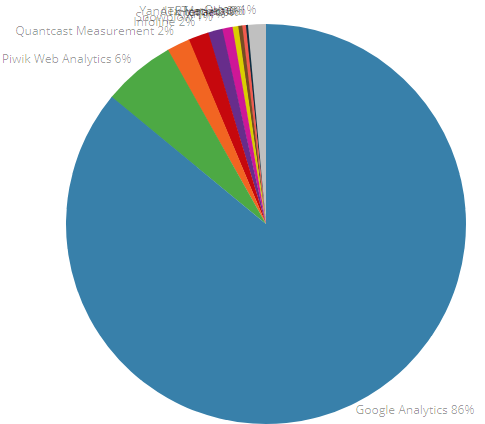
\includegraphics[width=0.45\textwidth,valign=t]{images/analysis/analytics-usage2}}
			\caption{Marché occupé par Google Analytics dans les domaines d'analyse, de tracking et de mesure d'audience sur le Web.}
			\label{analytics-usage}
		\end{figure}

		Nous pouvons calculer grâce au premier graphique que l'ensemble des produits de Google, y compris Google Analytics et ses versions proches, représentent plus de 83\% des installations de solutions dans le domaine de l'analyse et du tracking. De plus pour la sous-catégorie du marché de la mesure d'audience uniquement, Google Analytics a lui seul représente 86\% d'installations sur le Web.

		\begin{figure}[ht]
			\centering
			
\includegraphics[width=0.4\textwidth]{images/analysis/analytics}
			\caption{Logo de la solution Google Analytics\cite{analytics}.}
			\label{a-analytics}
		\end{figure}

		Il est donc de plus en plus évident que s'intéresser aux fonctionnalités de Google Analytics est intéressant pour les buts du projet. Nous souhaitons nous poser la question du risque encouru par les utilisateurs en se connectant sur un site web utilisant Google Analytics. Quelles informations sont prélevées ? Lesquelles sont envoyées ? Les données sont-elles anonymisées ?

	\subsection{Google Analytics}

		Google Analytics se présente comme une solution d'analyse de statistiques d'utilisateurs dans le but d'améliorer les résultats des sites web sur lesquels il est installé. Ce produit étant totalement gratuit pour les PME, il est aujourd'hui très répandu sur le net et particulièrement en Suisse\cite{analytics-usage}.

\section{Extensions de navigateur}

	\subsection{Introduction}

		Au vu de l'objectif du projet qui est à la fois de récolter des données tout en montrant un feedback à l'utilisateur, l'extension pour navigateurs est le moyen le plus facile à la fois pour nous de distribuer notre code, et pour les utilisateurs de l'installer. Cependant, de nombreuses extensions dont le but est de montrer des statistiques sur la navigation de l'utilisateur existent déjà. L'objectif n'est donc pas seulement d'implémenter les mesures adéquates pour notre étude, mais également de fournir des fonctionnalités à l'utilisateur novatrices afin que l'extension se démarque des concurrents.

		Une analyse des extensions existantes est donc requises afin de prendre des décisions sur la direction que vont prendre les fonctionnalités implémentées.

	\subsection{Etat de l'art}

		Nous nous intéressons aux extensions disponibles pour deux des navigateurs les plus utilisés : Google Chrome, et Mozilla Firefox. Chaque navigateur possède son propre éventail d'extensions, bien que parfois certaines se retrouvent disponibles dans les deux catalogues. Chrome Web Store\cite{chromewebstore} est le catalogue officiel d'extensions pour Google Chrome, et Modules Firefox\cite{modulesfirefox} est celui correspondant à Mozilla Firefox. Quelques recherches avec des mots-clé adaptés sur chaque catalogue vont nous fournir les extensions les plus populaires pour un thème semblable aux nôtre.

		\subsubsection{timeStats}

			timeStats\cite{timestats} est une extension disponible pour Google Chrome. La figure~\ref{a-timestats} montre comment l'extension se présente via une image montrée sur le Google chrome Store.

			\begin{figure}[h]
				\centering
				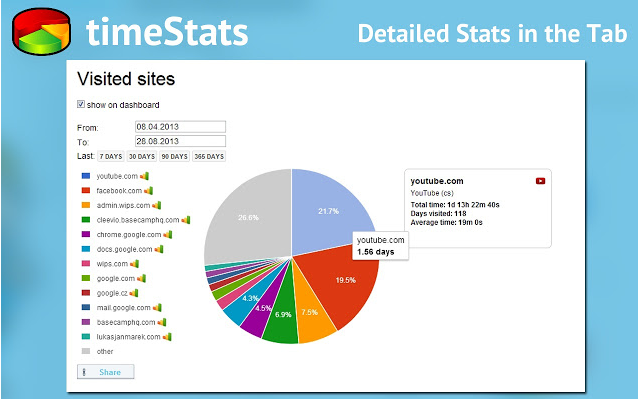
\includegraphics[width=0.6\textwidth]{images/analysis/timestats}
				\caption{Image de présentation de timeStats\cite{timestats}.}
				\label{a-timestats}
			\end{figure}

			Cette extension se focalise sur la visualisation du temps passé sur les différents sites web, parfois regroupés en domaines. La plupart des informations représentées sont le temps passé, et l'extension s'organise en plusieurs pages permettant de voir des visualisations différentes. On remarque la présence de plusieurs types de graphiques (en ligne, en secteurs) adaptés à la mesure affichée. timeStats est disponible pour Google Chrome uniquement.

		\subsubsection{Ghostery}

			Ghostery est une extension Google Chrome qui possède également sa propre page web en dehors du catalogue. La figure~\ref{a-ghostery} montre la page d'accueil du site ``ghostery.com'', qui est le domaine officiel de l'extension listée sur Google Chrome.

			\begin{figure}[h]
				\centering
				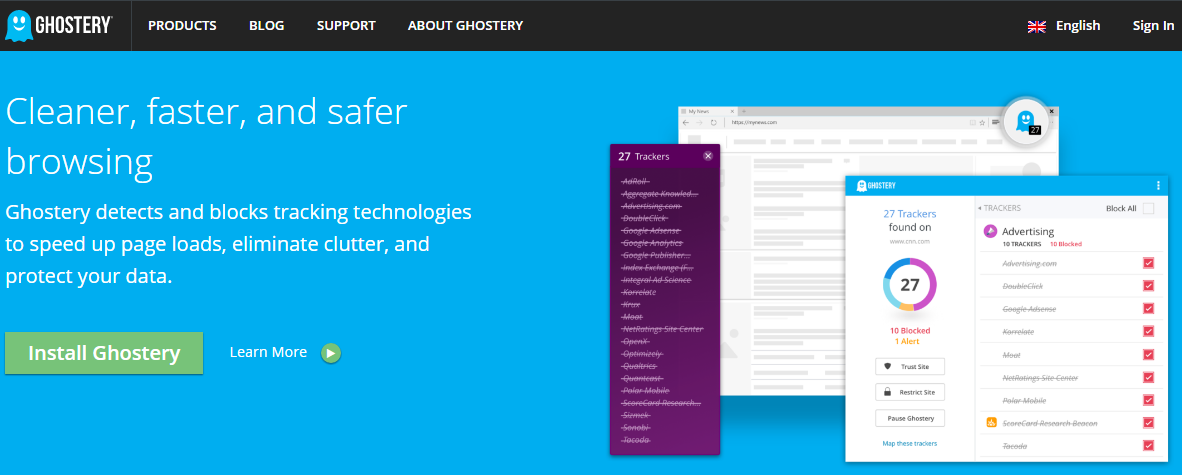
\includegraphics[width=0.8\textwidth]{images/analysis/ghostery}
				\caption{Page d'accueil de Ghostery\cite{ghostery}.}
				\label{a-ghostery}
			\end{figure}

			Ghostery semble donc se concentrer sur la détection et le blocage des informations envoyées aux trackers tiers lors de la navigation. Quelques options de personnalisation y sont présenter, comme la possibilité d'autoriser des trackers particuliers, ou des domaines choisis.

		\subsubsection{Privacy manager}

			Privacy manager se montre comme une extension permettant la gestion de mécaniques liées à la préservation de la vie privée. La figure~\ref{a-privacymanager} montre l'interface principale utilisée par l'extension.
			Bien que certaines options existent pour la protection de la vie privée, presque la moitié les options activables n'ont pas directement à faire avec la vie privée, et sont plutôt des désactivation ou activations de fonctionnalités de productivité.

			\begin{figure}[h]
				\centering
				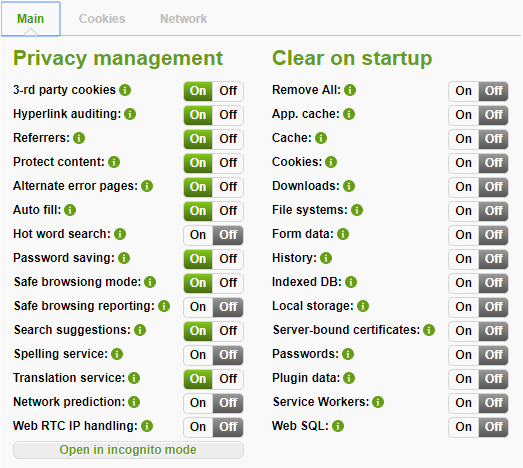
\includegraphics[width=0.5\textwidth]{images/analysis/privacy-manager}
				\caption{Interface de base de Privacy manager\cite{privacymanager}.}
				\label{a-privacymanager}
			\end{figure}

		\subsubsection{TheGoodData}

			TheGoodData remplit à priori la même mission que Ghostery, mais propose des outils légèrement différents, et son thème est centré sur l'utilisation de la valeur des données de navigation pour une bonne cause. Un tableau de bord montré à la figure~\ref{a-thegooddata} permet de se renseigner sur l'état actuel de sa navigation avec des analyses basiques sur les dangers trouvés.

			\begin{figure}[h]
				\centering
				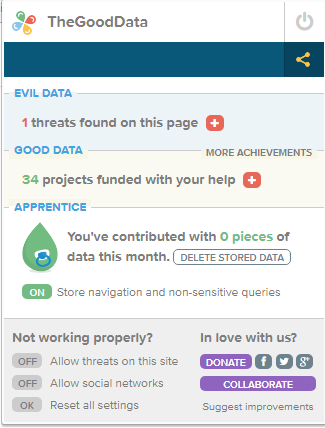
\includegraphics[width=0.4\textwidth]{images/analysis/thegooddata}
				\caption{Interface de TheGoodData\cite{thegooddata}.}
				\label{a-thegooddata}
			\end{figure}

		\subsubsection{Noiszy}

			\begin{figure}[h]
				\centering
				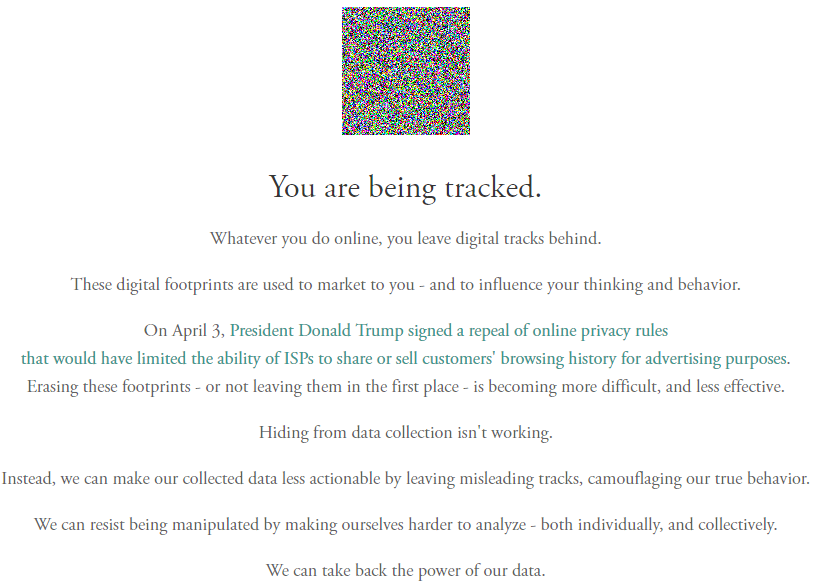
\includegraphics[width=0.9\textwidth]{images/analysis/noiszy}
				\caption{Premier paragraphe de la page web de Noiszy\cite{noiszy}.}
				\label{a-noiszy}
			\end{figure}

			Noiszy cherche quand à lui à brouiller les pistes des trackers existants, sans les bloquer. Son hypothèse de base est qu'il est presque impossible de dissimuler complètement ses "Digital Footprints", et que la meilleure solution est de tenter de les brouiller en les "falsifiant", par exemple en envoyant des données erronées aux trackers, ou en quantité trop élevées.
			La figure~\ref{a-noiszy} montre le premier paragraphe de présentation de Noiszy, présent sur leur site web.

		\subsubsection{Privacy Badger}

			Privacy Badger est une extension développée par l'EFF\cite{eff}. Disponible à la fois sur Google Chrome et Mozilla Firefox, cette extension a également comme objectif de contrôler l'envoi de données à des trackers.
			Plutôt que de strictement bloquer toute requête, cette extension laisse à l'utilisateur décider quel niveau de danger représenter chaque tracker, et adapte son comportement entre un blocage total, la retenue de certaines informations ou aucune action entreprise pour chaque tracker détecté.
			La figure~\ref{a-privacybadger} montre l'interface de l'application une fois celle-ci installée. On peut y voir les lignes de présentant chacune un tracker, et la possibilité de définir son niveau de danger, et par conséquent l'action appropriée associée.

			\begin{figure}[h]
				\centering
				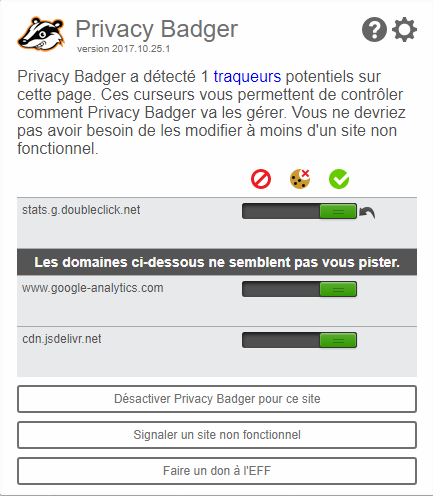
\includegraphics[width=0.5\textwidth]{images/analysis/privacybadger}
				\caption{Contrôle des actions face aux trackers de Privacy Badger\cite{privacybadger}.}
				\label{a-privacybadger}
			\end{figure}

		\subsubsection{Kraken.me}

			Kraken.me est une extension de navigateur, mais également une application pouvant s'installer sur smartphone. Cette application analyse le flux de données de certains services comme Facebook, Twister, LinkedIn et encore d'autres. L'objectif est ici de donner à l'utilisateur une vue sur ses propres données, et la manière que celles-si sont utilisées par les applications.
			La figure~\ref{a-krakenme} montre le modèle présenté par le site web.

			Cette application est probablement une des plus semblable à l'objectif général de notre projet, il serait donc intéressant de voir quels ont été les débouchés de cette étude. Notons que la plupart de l'activité de celle-ci ainsi que de l'outil semblent avoir cessé en 2014.

			\begin{figure}[h]
				\centering
				
\includegraphics[width=0.8\textwidth]{images/analysis/krakenme}
				\caption{Flux de données de Kraken.me\cite{krakenme}.}
				\label{a-krakenme}
			\end{figure}

	\subsection{Conclusion}

		Après avoir dressé une liste des extensions de navigateur les plus populaires et utilisés, nous pouvons prendre position sur les fonctionnalités que notre extension va posséder afin de se démarquer et de répondre à la problématique de l'étude. Nous allons choisir les fonctionnalités que nous estimons avoir un impact pour la sensibilisation du public aux traces que les internautes laissent, et des informations que nous pouvons en retirer. Ainsi, le plug-in se concentrera sur les deux aspects suivants :

		\begin{itemize}
			\item Détection et mise en lumière des différents trackers présents sur les pages visitées par l'utilisateur.
			\item Tentative de reconstitution du profil de l'utilisateur à partir de la fréquence de la visite des pages web et de leur contenu.
		\end{itemize}

\section{Analyse de texte}

	Nous allons utiliser le contenu des pages pour trouver des informations sur les centres d'intérêt de l'utilisateur. Pour ceci, nous avons besoin d'analyser et de tenter de comprendre le contenu des pages.

	\subsection{Keyword extraction}

		Le keyword extraction est le nom donné à un algorithme dont le but est de ressortir, parmi les mots d'un document, quels en sont les mots les plus représentatifs, ou les plus expressifs. Cette opération ne se fait généralement pas sur un seul document, mais sur un ensemble de documents, appelé corpus. Il s'agit d'une sous-catégorie des algorithmes de \gls{NLP}.

		Dans notre cas, les techniques de keyword extraction que nous prenons en compte sont les techniques dites "non supervisées". Cela signifie que nous n'avons pas d'information à priori sur quels sont les mots qui vont être potentiellement importants dans le texte, et que nous laissons une complète liberté à l'algorithme.

		Parmi les techniques de keyword extraction, on peut citer les plus connus : \gls{TF-IDF}, TextRank et \gls{RAKE}. Etant donné que ces algorithmes fonctionnent de manière semblable, il a fallu se pencher sur des études montrant leur efficacité afin de décider lequel de ceux-ci nous allons utiliser.

		\subsubsection{Recherche}

			Etant donné qu'il s'agit ici d'entraîner des modèles à l'aides d'algorithmes non-supervisés, il n'existe pas de méthode efficace cartésienne pour prouver que nous obtenons des bons résultats à l'aide des modèles générés. Nous ne cherchons ici une vérité absolue, mais nous voulons trouver des modèles dans les pages parcourues par l'utilisateur. Les publications étudiées font donc également souvent appel à un jugement humain afin de définir si une méthode est adaptée ou non.

			Un total de trois ressources a été étudié pour baser notre choix de la technique de keyword extraction à utiliser.

			\paragraph{Première étude}
			
				La première source\cite{text-analysis-src4} présente un cas concret où on cherche à classifier une série de documents connus à l'avance, présentant des sujets communs. Le but est de créer un modèle capable de reconnaître le thème de nouveaux documents  en créant un modèle à partir d'une liste de documents connus. Bien que la comparaison soit faite entre TF-IDF, RAKE et TextRank, le cas ici assez différent du nôtre. En effet, le cas décrit ici cherche à entraîner un modèle de manière supervisée. 

				L'ensemble des documents en entrée est une liste de documents lus par l'auteur de l'article durant les 6 dernières années. Après avoir testé les trois algorithmes et comparé les différents résultats, la conclusion est que pour ce cas, TextRank et RAKE sont les algorithmes préférables. Le reproche est fait à TF-IDF de classer trop bas certains mots qui apparaissent dans de nombreux documents. Par exemple, nous savons que l'auteur a lu beaucoup de document sur JavaScript, et donc TF-IDF met un poids très faible à ce mot.

				Cette conclusion est sensée, mais ce problème ne s'applique pas à notre cas. En effet, nous cherchons spécifiquement à avoir un éventail très large de pages afin d'éviter ce genre de cas. Également, notre entraînement ne sera pas supervisé, nous ne pourrons donc pas évaluer les résultats finaux de cette manière.

			\paragraph{Deuxième étude}

				La deuxième étude\cite{text-analysis-src5} se penche sur l'extraction automatisée et non supervisée de keywords, ce qui est cette fois très proche de notre cas. Cette fois-ci, la publication se base sur des méthodes statistiques pour tenter de prédire quel est l'algorithme le plus efficace pour le keywords extraction en comparant les résultats de ceux-ci avec l'avis d'humains auxquels ont demande d'exécuter la même tâche.

				Sont comparées ici la méthode TF-IDF ainsi que certaines de ses variantes, et plusieurs méthodes basées sur l'utilisation de graphes (référées simplement comme "Graph-based methods" à plusieurs endroits du texte).

				Après une comparaison des résultats de chaque méthode avec les résultats trouvés par des humains, il est conclu que "Our results on the human transcripts show that the simple TFIDF based method is very competitive"\cite{text-analysis-src5}. Certaines variantes de TF-IDF où la position des mots dans une phrase ajoute un poids aux mots offre des scores très comparables à la méthode de base, mais les autres techniques ont montré des résultats plus faibles.

			\paragraph{Troisième étude}

				Le troisième document\cite{text-analysis-src6} est en réalité une question posée sur le site Quora, où des experts ont proposé une réponse à la question "What are the best keyword extraction algorithms for natural language processing and how can they be implemented in Python?".

				Les trois méthodes populaires \gls{TF-IDF}, TextRank et \gls{RAKE} sont à nouveau citées, mais il ressort que RAKE et TF-IDF semble être consensuellement les méthodes les plus efficaces.

			À la fin de l'analyse de ces sources, nous choisissons d'utiliser l'algorithme TF-IDF, qui semble être à la fois efficace et adapté à notre cas.

		\subsection{TF-IDF}\label{analyse-tfidf}

			TF-IDF est une méthode attribuant un poids à chaque mot de chaque document d'un corpus. Ce poids mesure l'importance relative du mot dans ce document. Le nom "TF-IDF" signifie "Term Frequency - Inverse Document Frequency". Le poids final d'un mot dans un document se calcule en prenant en compte uniquement deux mesures :
			\begin{description}
				\item[TF] Term Frequency : La quantité d'apparition de ce mot dans ce document
				\item[DF] Document Frequency : Le nombre de documents dans lesquels ce mot apparaît
			\end{description}

			Le score final d'un mot multiplie le TF d'un mot à l'inverse de son DF. Cela signifie que pour avoir une grande importance dans un document, un mot sera typiquement :
			\begin{itemize}
				\item Présent de nombreuses fois dans ce document
				\item Présent dans très peu d'autres documents
			\end{itemize}

			Le calcul des poids se fait sur l'ensemble du corpus en une fois, car il nécessite que l'on connaisse le nombre d’occurrences de chaque mot dans l'entièreté du corpus de documents. Il n'est donc pas possible de mettre à jour les poids de manière "online" en utilisant ce modèle.

	\subsection{Topic Modeling}

		Le topic modeling est un exercice différent de celui du keyword extraction. Nous ne cherchons plus ici à trouver les meilleurs mots parmi des textes, mais nous cherchons à les regrouper afin d'en former des thèmes, ou "topic"s.

		Le but est cette fois de déterminer par des méthodes statistiques quels sont les thèmes communs à plusieurs documents, nous permettant ainsi de les regrouper. Ceci part du principe que nous appliquons l'apprentissage de l'algorithme sur un corpus de documents qui contient des textes qui ont effectivement des thèmes en commun. Ce qui est sans doute notre cas lorsque notre corpus est composé de pages web visitées par des utilisateurs.

		\subsubsection{Recherche}

			Etant donné que nous sommes dans le même cas que TF-IDF, à savoir en recherche d'un algorithme pour le cas d'un apprentissage non supervisé, la plupart des méthodes tentant de comparer des modèles se basent sur des mesures empiriques. Le jugement humain est à nouveau indispensable dans ce cas pour déterminer de l'adéquation d'un algorithme ou non avec les buts recherchés.

			Nous recherchons ici une méthode relativement populaire car nous allons nous baser sur une librairie l'implémentant déjà. Il aurait été possible de développer nous-même ce module, mais nous avons estimé que les efforts à déployer pour ce faire étaient trop élevés pour justifier le temps passé.

			Après quelques recherches sur le web, les méthodes les plus populaires semblent être LSA, pLSA et LDA\cite{stanford-topicmodel}. Cependant, les études comparatives entre ces méthodes semblent très rares, et les seules sources trouvées furent des déclarations de chercheurs. Voici les ressources ayant contribué au choix de la méthode :

			\paragraph{Première source} 

				La première source comparant ces algorithmes est une réponse à une question posée sur le site web Quora\cite{quora-topicmodel}. À la question "What's the difference between Latent Semantic Indexing (LSI) and Latent Dirichlet Allocation (LDA)?", la réponse votée le plus positivement par un consultant en NLP conclut "In practice, LSI is much faster to train than LDA, but has lower accuracy.".

			\paragraph{Seconde source}

				La deuxième source est une question posée sur le site Reddit, intitulée "LSA vs pLSA vs LDA"\cite{reddit-topicmodel}. L'auteur demande la différence et les avantages de chaque méthode, et une réponse résume chaque algorithme en une simple ligne :
				\begin{quote}
LSA -> uses SVD, and as a result the topics are assumed to be orthogonal.

pLSA -> Treats topics as word distributions, uses probabilistic methods, and topics are allowed to be non-orthogonal.

LDA -> similar to pLSA, but with dirichlet priors for the document-topic and topic-word distributions. This prevents over-fitting, and gives better results.
				\end{quote}

				Semblablement, le modèle LDA semble primer dans l'avis sur la qualité des résultats. Après une recherche de librairies, il se trouve que LDA possède une implémentation en Python, dans une librairie nommée gensim. Nous nous arrêtons donc sur ce choix, comme le modèle semble à la fois précis et adapté à notre cas d'utilisation avec Python.

	\subsection{LDA}\label{analyse-lda}

		LDA (de l'anglais Latent Dirichelet Allocation) est un modèle de topic modeling, et va nous permettre de révéler des topics relatifs aux pages visitées par les utilisateurs. Ici, un topic est définit par une liste de mots, et un poids associé à chaque mot pour le topic.

			La génération d'un modèle LDA prend plusieurs paramètres en entrée, mais le plus important pour nous est de définir un nombre de topics que nous souhaitons voir en sortie. On fixe ce nombre de topics, puis on lance l'apprentissage du modèle sur l'ensemble du corpus de documents, opération que peut durer plusieurs heures.

			À la fin de l'apprentissage, nous sommes en possession d'un modèle que nous pouvons questionner de plusieurs manières, par exemple :
			\begin{itemize}
				\item Quels sont les mots les plus contribuant à un topic ?
				\item Quels sont les topics les plus probables pour un document ?
			\end{itemize}

			Nous allons donc par exemple utiliser le modèle afin d'assigner des topics au contenu d'URLs, et ainsi tenter de trouver quels sont les thèmes communs aux pages visitées par un utilisateur.
\chapter{Prototype 1}
%%%%%%%%%%%%%%%%%%%%%%%%%%
%                          %
% ----- INTRODUCTION ----- %
%                          %
%%%%%%%%%%%%%%%%%%%%%%%%%%

\section{Fonctionnalités}

	La première itération de l'application vise à couvrir certaines des exigences fonctionnelles demandées :
	\begin{itemize}
		\item Fenêtre avec liens dirigeant vers les pages
		\item Page "Cases" affichant la liste des cas avec possibilité d'afficher/cacher des colonnes, et de filtrer des lignes
		\item Page "Patients" affichant la liste des patients avec possibilité d'afficher/cacher des colonnes, et de filtrer des lignes
	\end{itemize}

\section{Conception}

	Le premier prototype de l'application a défini beaucoup des comportements et des mécaniques d'interaction de l'application.

	\subsection{Architecture générale de l'application}

		Tout d'abord, il était nécessaire de réfléchir à l'architecture générale de l'application avant de s'attaquer à chaque partie. Au vu du produit demandé, l'application sera réalisée suivra une architecture classique du schéma Client - Serveur. Du code se trouvera donc exécuté sur le client, et sur le serveur.

	\subsubsection{Frontend}

		La partie frontend est développée à l'aide de React. Il s'agit d'une one-page app : Cela signifie que l'utilisateur utilisera toujours la même adresse web pour accéder à l'application : Celle-ci se chargera ensuite elle-même de se transformer en les diverses interfaces que l'utilisateur va demander.

		Cette page est développée à l'aide de React et de librairies permettant de compléter React, et la structure du code suivra une architecture adaptée à l'utilisation de Flux, dont nous avons parlé précédemment. Il s'agit de l'architecture qu'il est recommandé d'utiliser avec React pour une application de taille moyenne, ce qui correspond à notre projet.

	\subsubsection{Backend}

		La partie backend se compose d'une couche applicative ainsi que d'une base de données. Le client ayant déjà crée une base de données de type MySQL avant le début du projet, elle ne sera pas changée.

		La partie applicative du backend est développée en node.js. Ce choix s'est fait pour des raisons de simplicité : Etant donné que la partie frontend du projet est développée à l'aide d'outils adaptés pour JavaScript, il est assez naturel de continuer le développement du backend avec des technologies similaires.

		La partie base de données restera donc avec MySQL. Quelques changements à la structure de la base de données seront apportés afin que celle-ci soit totalement compatible avec l'application demandée.

	\subsection{Structure de la navigation}

		En plus de répondre aux demandes du client, le but est de concevoir une application qui soit facile et agréable d'utilisation.
		Il a donc été nécessaire de réfléchir à la structure de la navigation de l'application en elle-même, ainsi qu'aux interactions qu'elle propose à l'utilisateur.

		L'analyse des différentes parties de l'application a mené à une compréhension des différentes pages à mettre en place afin de répondre aux besoins des différents clients.

		\paragraph{Cases} La page \textit{Cases} va présenter une vue des différents Cas. Un cas est lié à une épaule d'un patient, et à un ou plusieurs scans. Cette page va présenter dans un tableau la liste de tous les cas. Cette liste pourra être ordonnée et triée selon plusieurs critères. Il s'agira de la page que va principalement utiliser de public de la catégorie "scientifique". Un clic sur un cas ouvrira une page avec toutes les informations détaillées sur ce cas, comprenant entre autres des visualisations de scans.
		\paragraph{Patients} La page \textit{Patients} va présenter une vue de tous les patients. Cette page sera utilisée principalement par le public de la catégorie "clinique". Elle va présenter une liste complète des patients. Cette liste pourra également être ordonnée et filtrée selon plusieurs critères. Un clic sur un patients ouvrira une page montrant de manière détaillée les informations du patient, ainsi que l'ensemble des cas qui lui appartient. De là, il sera possible de naviguer sur un cas en particulier.
		\paragraph{Studies} Cette page va montrer un ensemble d'études faites sur les données de la base.
		\paragraph{Stats} Cette page va montrer des statistiques sur les données médicales des patients.
		\paragraph{Informations} Cette page va présenter de manière statique des informations sur le projet d'une manière générale.
		\paragraph{Admin} Cette page offrira un panel d'administration de l'outil. Les fonctionnalités de celui-ci ne sont pas encore totalement définies.

		La figure \ref{structure_navigation} montre l'ensemble des pages ainsi que leur hiérarchie.

		\begin{figure}[h]
			\centering
			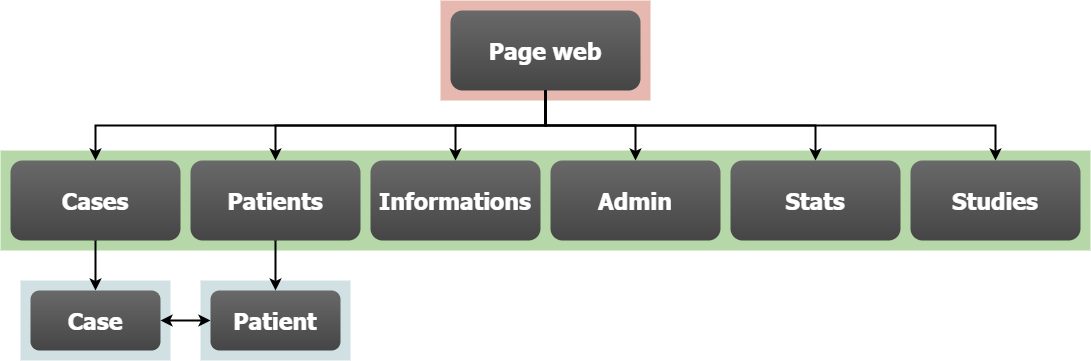
\includegraphics[width=1\textwidth]{images/conception/structure_navigation}
			\caption{La structure de la hiérarchie et navigation entre les vues}
			\label{structure_navigation}
		\end{figure}

	\subsection{Maquettes}

		Des maquettes de l'interface ont été réalisées dès le début du projet. Celles-ci ne sont typiquement pas totalement fidèles à ce que ressemblera la solution finale ; le but est de montrer la structure de la navigation, ainsi que se donner les moyens de les améliorer sur le temps et de s'assurer que l'on comprenne les features demandées. La figure~\ref{maquette_papier} montre par exemple la toute première ébauche de la page des cas, et la figure ~\ref{maquette_papier2} montre la même version de la vue d'un cas particulier.

		\begin{figure}[!h]
			\centering
			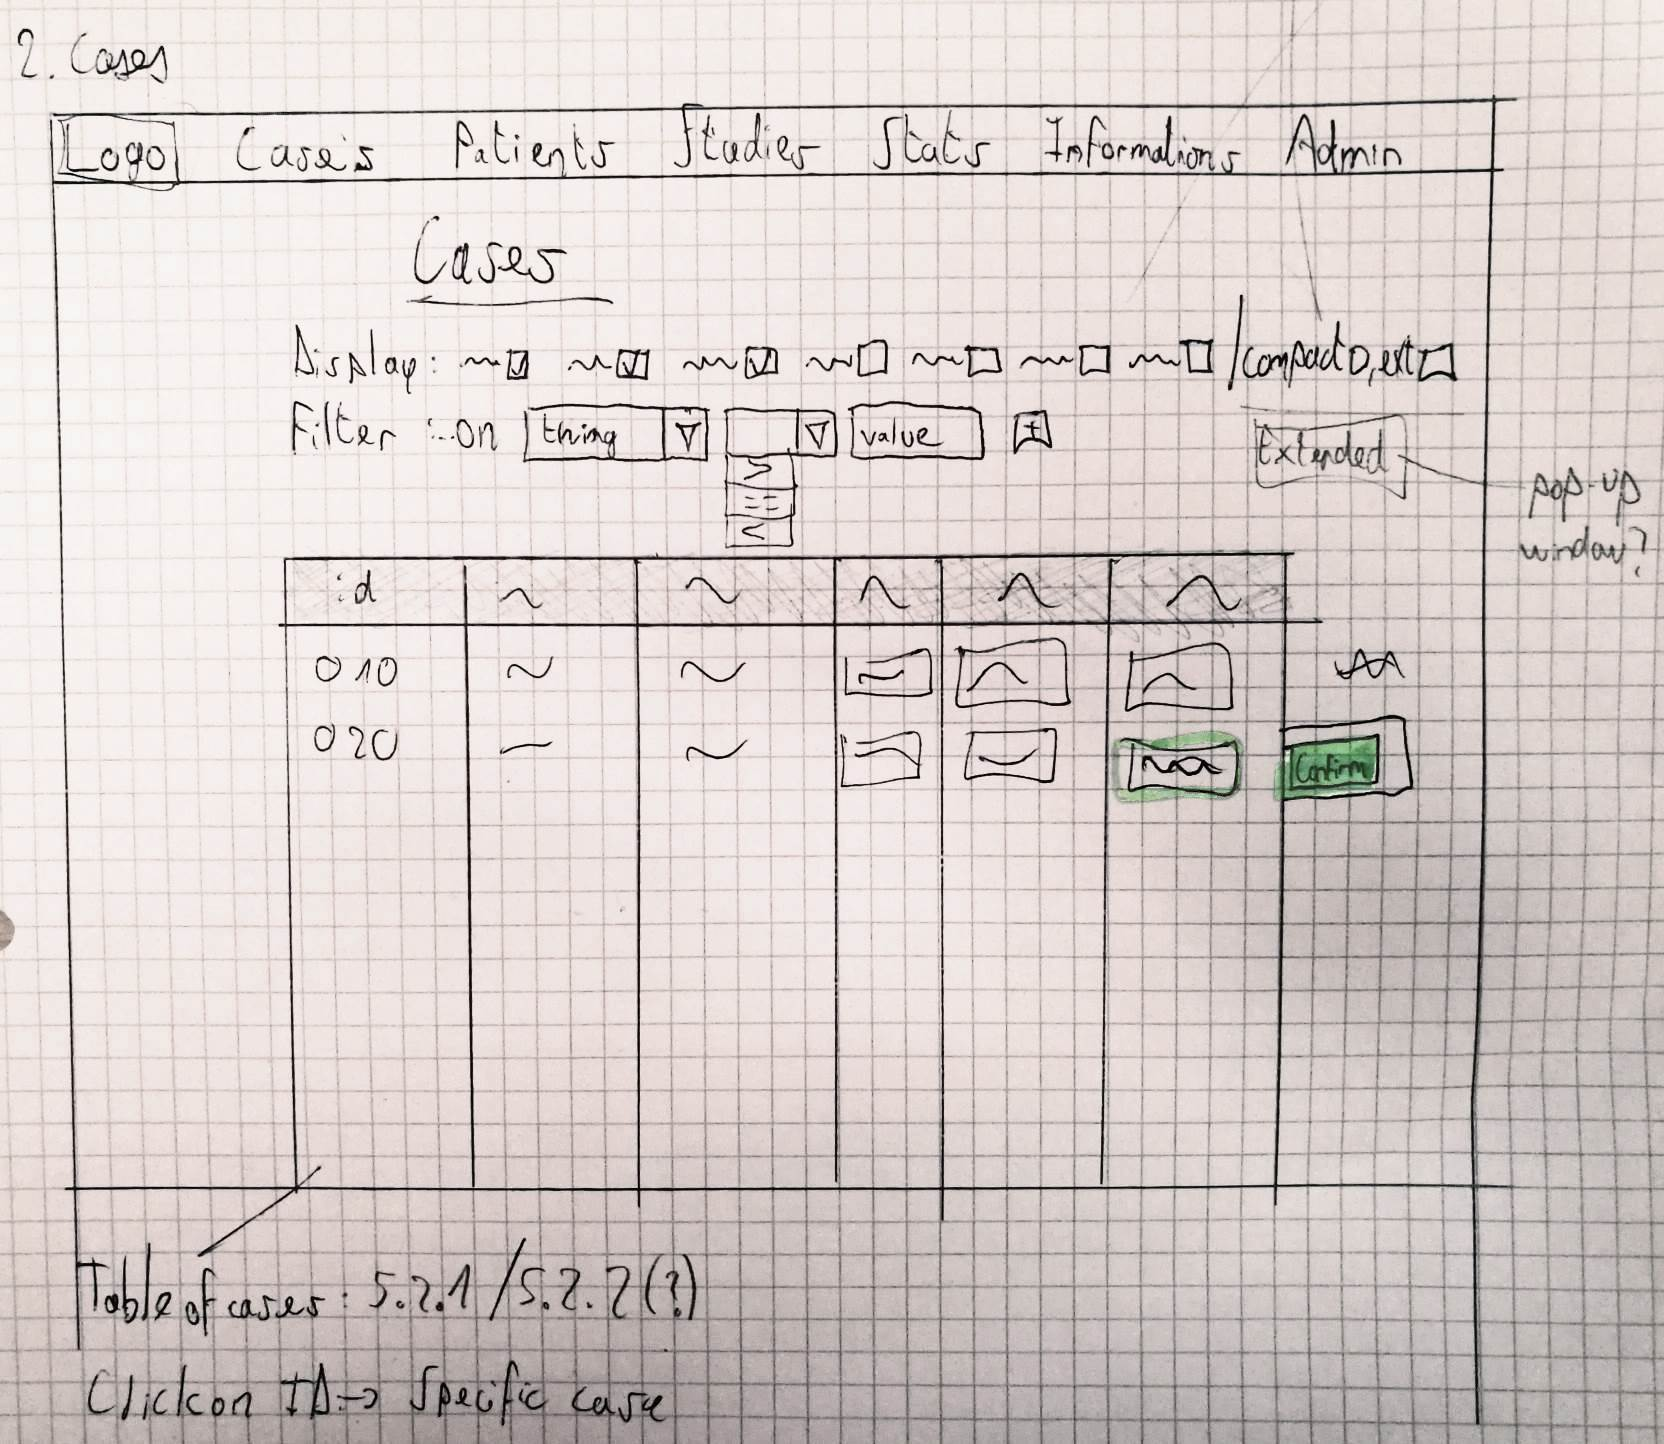
\includegraphics[width=1\textwidth]{images/analyse/maquette1}
			\caption{Wireframe sur papier de l'interface de la liste des cas}
			\label{maquette_papier}
		\end{figure}

		\begin{figure}[!h]
			\centering
			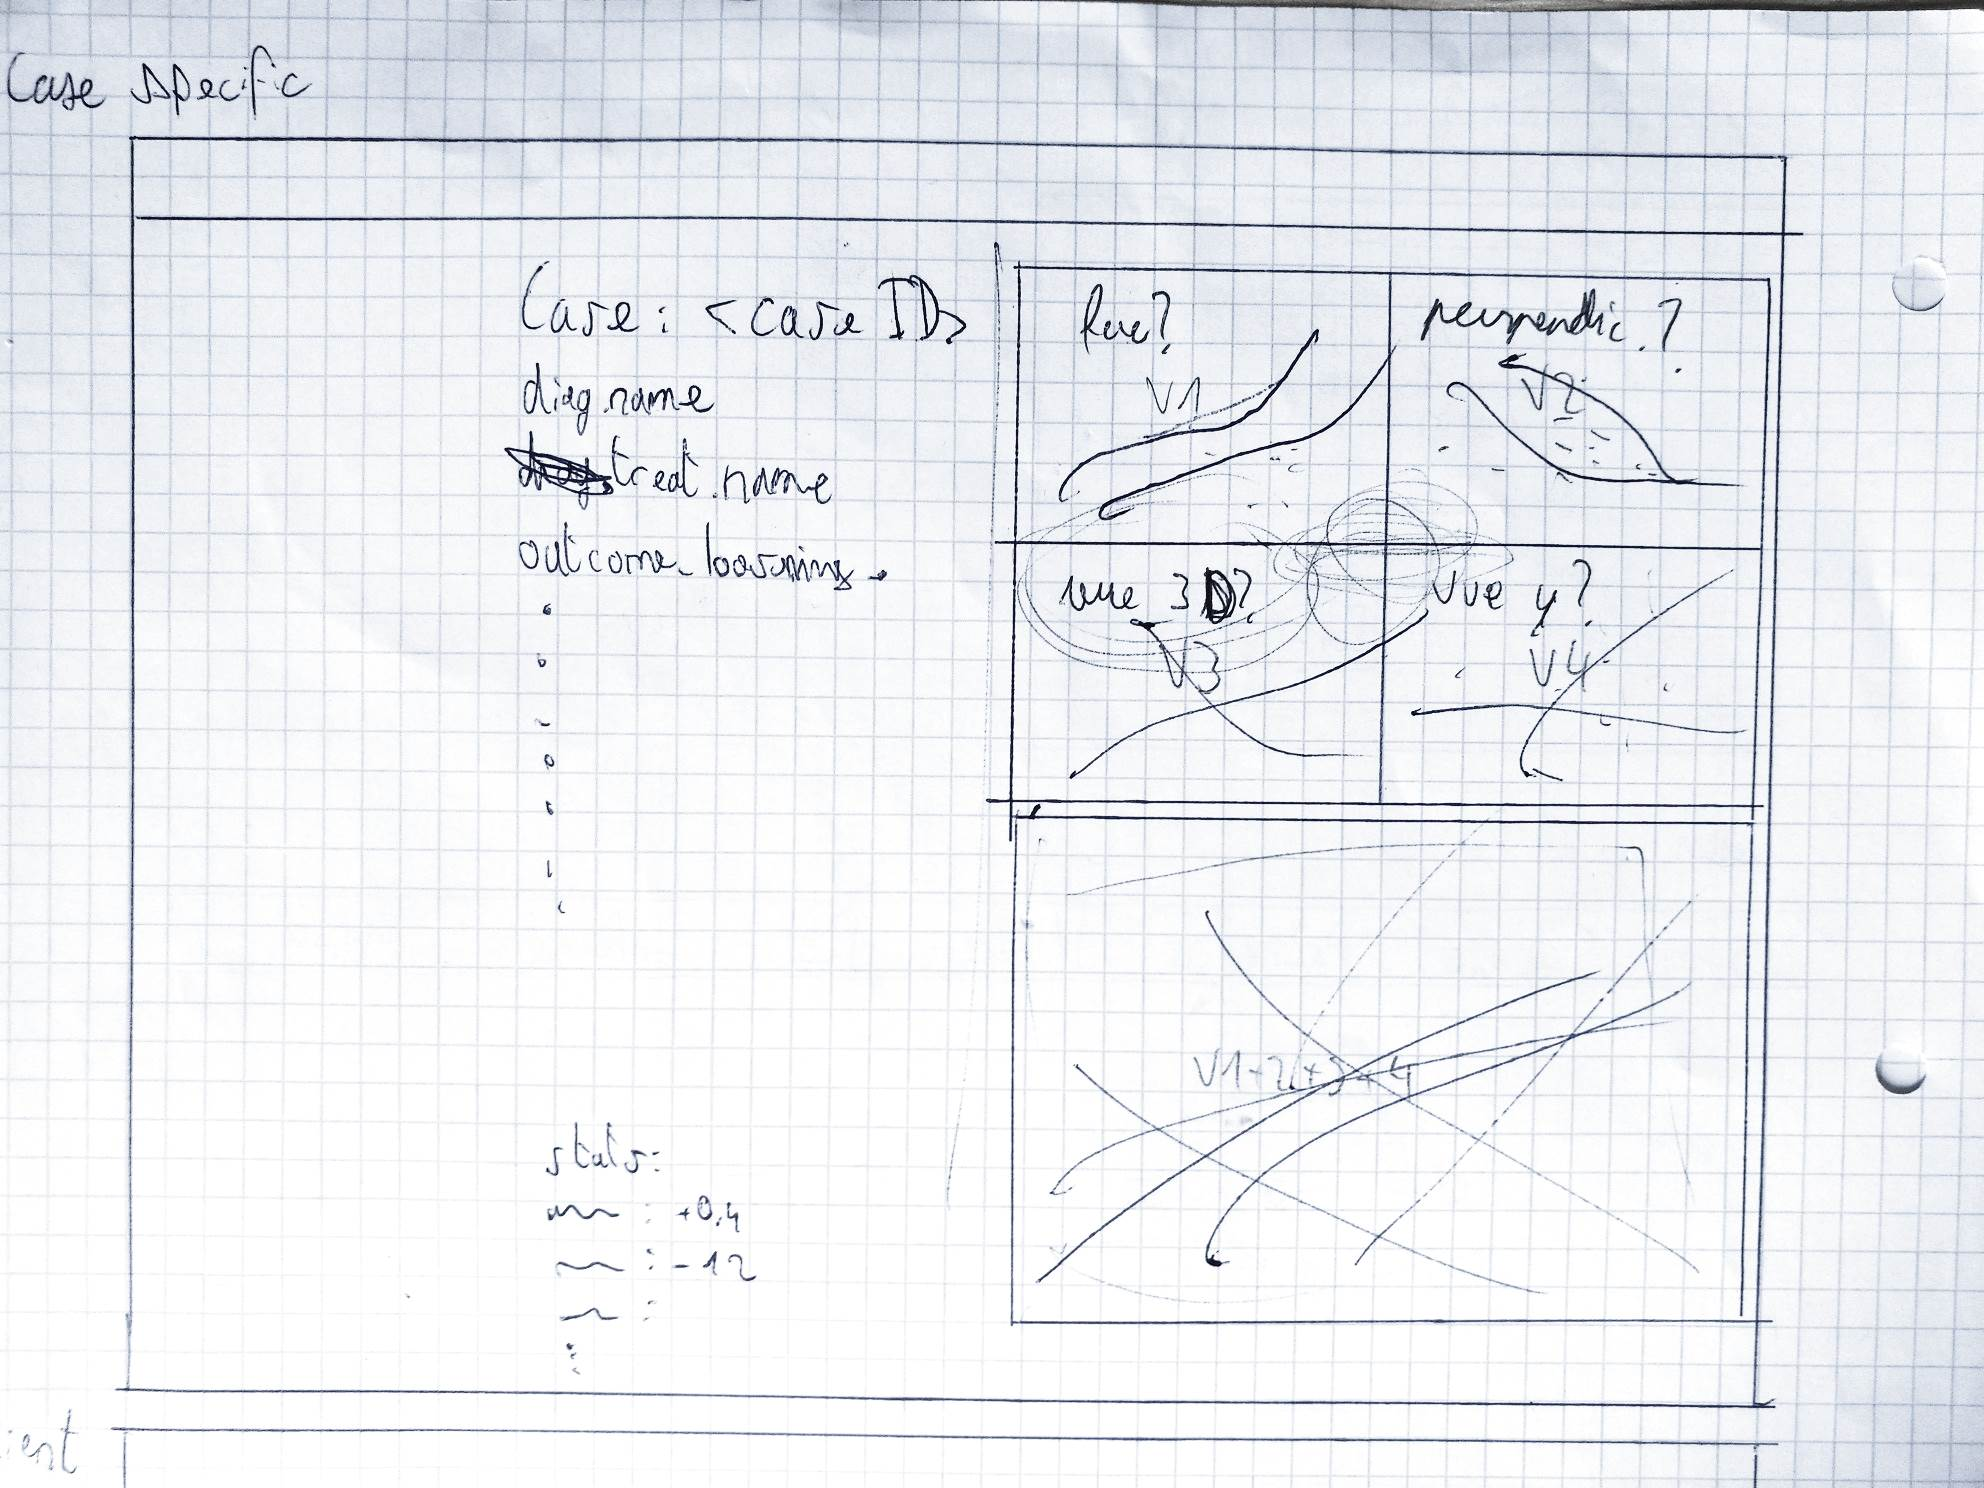
\includegraphics[width=1\textwidth]{images/analyse/maquette2}
			\caption{Maquette sur papier de l'interface d'un cas particulier}
			\label{maquette_papier2}
		\end{figure}

		La figure \ref{maquette_papier3} montre un sketch de deux pages secondaires au projet : une page d'administration ainsi qu'une page de statistiques.

		\begin{figure}[!h]
			\centering
			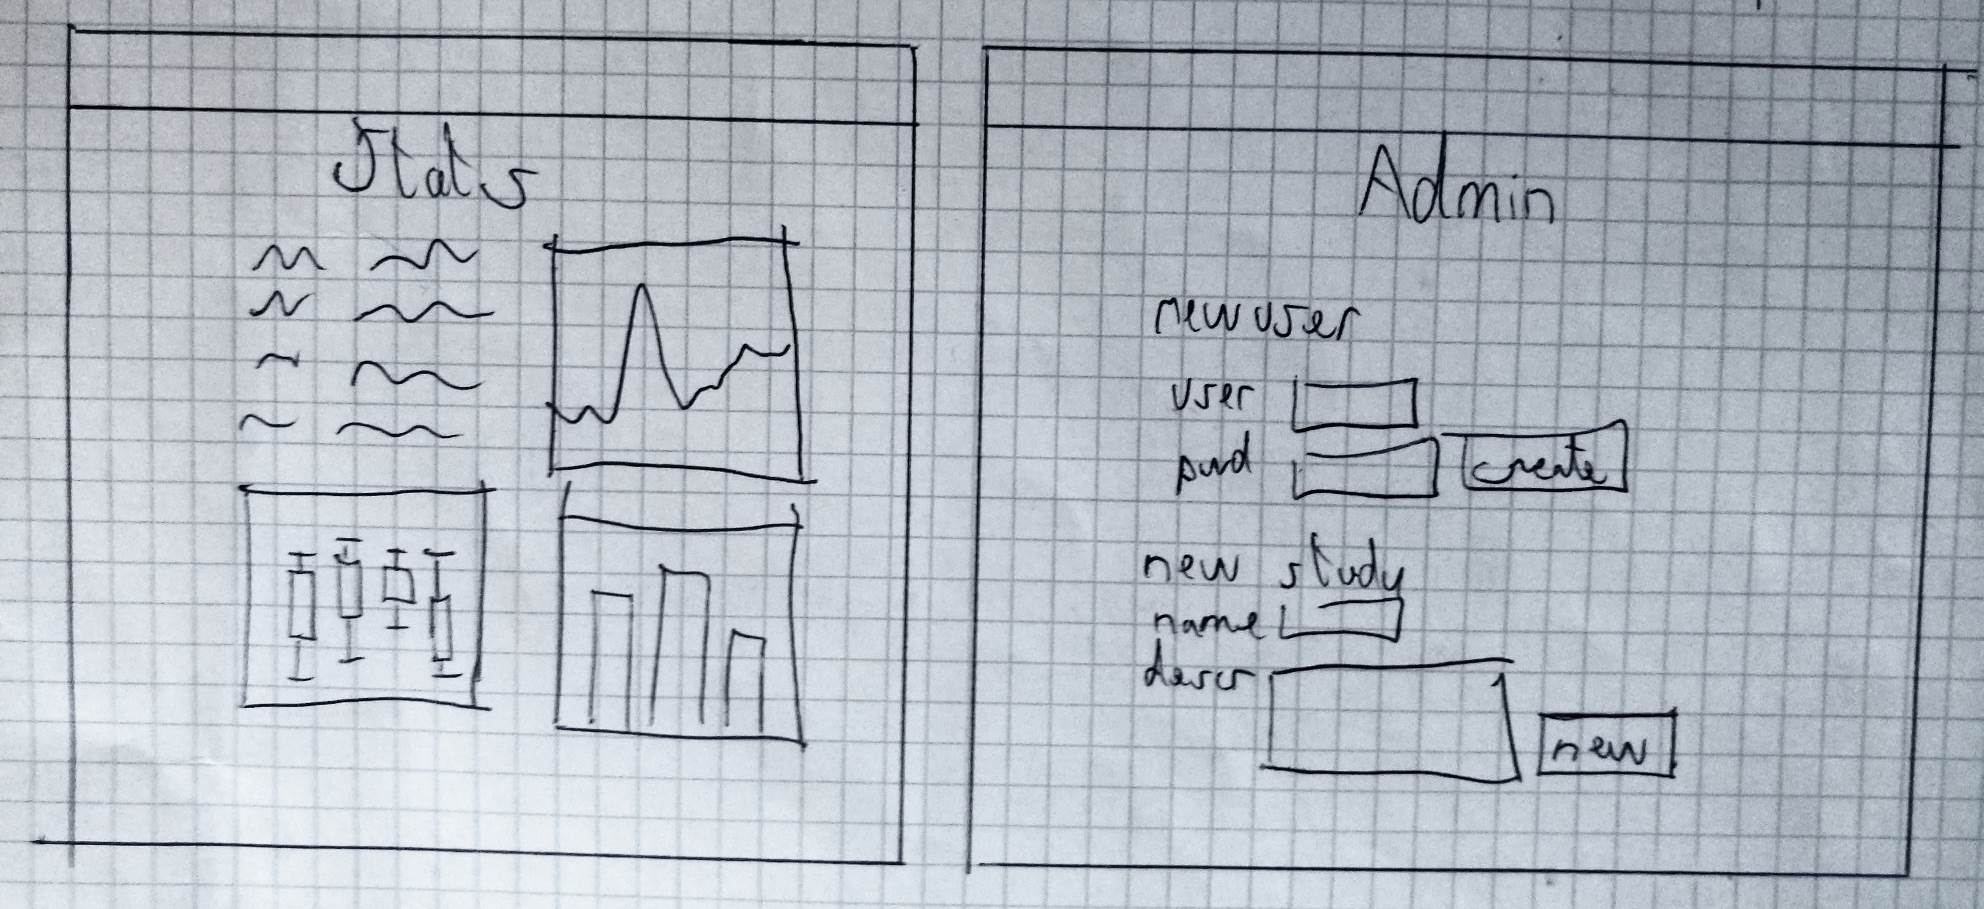
\includegraphics[width=1\textwidth]{images/analyse/maquette3}
			\caption{Sketch sur papier des pages "Stats" et "Admin"}
			\label{maquette_papier3}
		\end{figure}

\section{Implémentation frontend}

	L'implémentation du frontend a commencé par le choix et l'installation de l'environnement et des outils nécessaires pour développer en React de manière efficace. Le chapitre \ref{techno-react} explique l'utilité de chacun des composants, mais nous allons nous simplifier le travail en utilisant une configuration déjà prête pour le développement en React. Celle-ci est tirée du code annexe à la série de tutoriels suivis. Le code de cette configuration est disponible sur GitHub \cite{react-boilerplate}, et il s'agit de la configuration que j'ai utilisée. Tout le code décrit plus tard repose donc sur cette configuration.

	Le premier prototype s'est concentré sur l'implémentation des aspects qui ont été estimés comme étant centraux à l'application. Voici une liste des fonctionnalités du côté frontend qui doivent être implémentées pour réaliser le prototype :

	\begin{itemize}
		\item Disposition générale des éléments de la page
		\item Routage de chaque page sur sa vue correspondante
		\item Implémentation des pages "Patients" et "Cases"
		\item Lien avec les données de la base de données
	\end{itemize}

	\subsection{Disposition générale des éléments sur la page}

		Avant de démarrer à organiser les éléments d'une page, il est d'abord essentiel d'organiser les informations qui sont communes à toutes les pages. Comme le montre la figure \ref{maquette_papier}, il est prévu de naviguer entre les pages via une barre contenant les liens des autres vues, et qui se situe en haut de la page actuelle. 

		Toutefois, la décision a été prise de respecter au maximum les guidelines de Material Design\cite{material-design-guidelines}. Ici, il est préconisé d'utiliser une barre vertical contenant les liens vers les vues, appelée ``\texttt{Drawer}''. Ce Composant est d'ailleurs disponible dans la librairie Material-UI, mais il n'a pas pu être utilisé directement car il ne permet pas d'être continuellement visible. Dans ce cas ainsi que comme dans plusieurs cas dans le reste de l'application, il est nécessaire de l'implémenter en utilisant uniquement le CSS fourni par Material Design.

		Les liens vont donc rester sur la gauche de la page, et la vue principale sera affichée dans la partie droite.

		\begin{figure}[!ht]
			\centering
			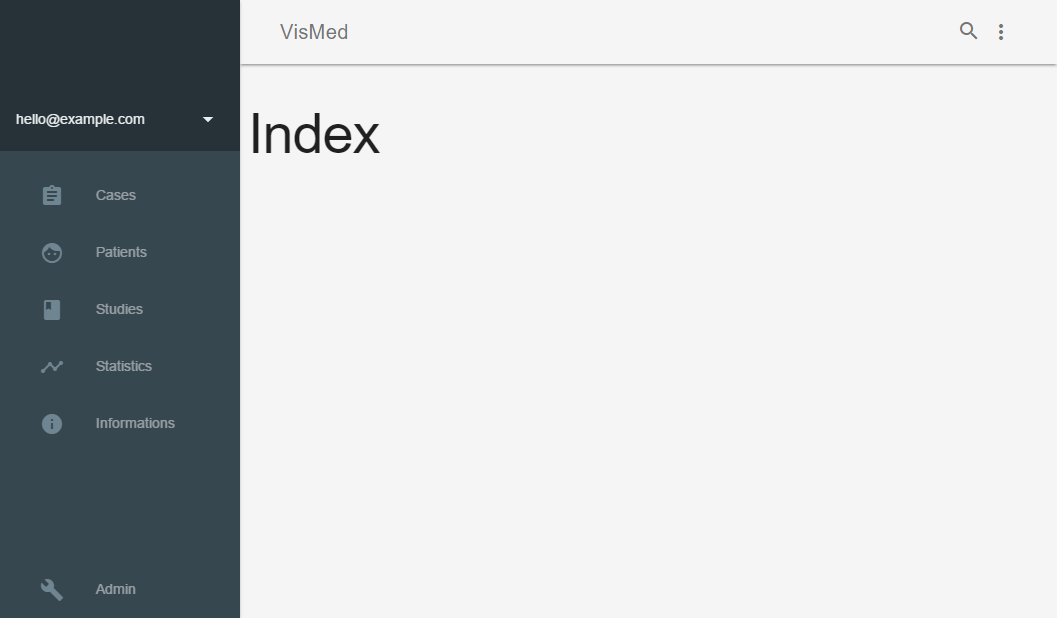
\includegraphics[width=1\textwidth]{images/realisation/proto1_1}
			\caption{Premier prototype fonctionnel de l'application}
			\label{proto1_1}
		\end{figure}

		La figure \ref{proto1_1} montre une des premières versions de la page, avec les liens du menu à gauche de celle-ci.

	\subsection{Routage}

		Etant donné que le but est de réaliser une "one-page app", nous allons utiliser une méthode de routage bien intégrée à React. Plutôt que télécharger une vue depuis le serveur à chaque fois que l'on désire changer de page, l'application entière est téléchargée au lancement de la page, et le changement de vue ainsi que le routage des liens se fait du côté client.

		Cet effet est accompli à l'aide de la librairie React-Router\cite{react-router}. Elle permet de déclarer quel Composant doit s'afficher en fonction de l'URL demandée, et de naviguer entre les vues sans rafraîchir la page complète.

\begin{figure}[!h]
\begin{lstlisting}[language=html]
<Router>
  <MuiThemeProvider muitheme={muiTheme}>
    <div class="mdl-layout_container">
      <div class="demo-layout mdl-layout mdl-js-layout mdl-layout--fixed-drawer mdl-layout--fixed-header">
        <Header/>
        <Aside/>
        <main class="mdl-layout__content mdl-color--grey-100">
          <div class="mdl-grid demo-content">
            <Route path="/" exact={true} name="index" component={Index}></Route>
            <Route path="/cases" name="cases" component={Cases}></Route>
            <Route path="/patients" name="patients" component={Patients}></Route>
            <Route path="/studies" name="studies" component={Studies}></Route>
            <Route path="/statistics" name="statistics" component={Statistics}></Route>
            <Route path="/informations" name="informations" component={Informations}></Route>
            <Route path="/admin" name="admin" component={Admin}></Route>
          </div>
        </main>
      </div>
    </div>
  </MuiThemeProvider>
</Router> \end{lstlisting}
\caption{Uutilisation des composants \texttt{Router} et \texttt{Route}}
\label{router-component}
\end{figure}

		La figure \ref{router-component} montre comment est déclaré le Router, ainsi que les différentes Routes de l'application. Le composant \texttt{Router} se trouve tout en haut de la hiérarchie, et c'est à l'intérieur de lui que les autres composants vont se placer. On peut voir qu'il n'y a aucun problème à mélanger du HTML (comme aux lignes 3 et 4) avec des composants React. Ce morceau de code représente à peu de choses près tout ce qui sera affiché sur les pages de l'application. Voici une liste des composants qu'on y trouve, et leur utilité :

		\begin{description}
			\item[\texttt{Router}] Englobe tous les composants devant pouvoir s'afficher ou se cacher selon l'URL demandée. Il doit donc englober toutes les \texttt{Route}s de l'application.
			\item[\texttt{MuiThemeProvider}] Nécessaire pour l'utilisation de la librairie Material-UI. Doit englober tous les éléments désirant utiliser des composants de cette librairie.
			\item[\texttt{Header}] Barre horizontale se trouvant au haut de la page. Affiche le titre de la page actuellement visitée.
			\item[\texttt{Aside}] Barre à gauche de la page, contenant les liens vers les différentes vues.
			\item[\texttt{Route}] Définit une route associée à une URL particulière, et quel composant afficher dans le cas où l'URL correspond à cette Route.
		\end{description}

		On voit donc ainsi que chaque Route va permettre d'afficher une page particulière. Par exemple, la ligne 10 traite le cas où l'URL se termine par \texttt{/cases}, et va donc se charger d'afficher le composant \texttt{Cases} à cet endroit. Chaque composant référencé par une \texttt{Route} (\texttt{Index}, \texttt{Cases}, \texttt{Patients}, \texttt{Studies} etc...) affiche donc sa vue lorsqu'il est appelé par le Router.

	\subsection{Pages "Patients" et "Cases"}

		Dans ce prototypes, les pages "Patients" et "Cases" sont très similaires. La figure montre la vue de la page "Patients".

		\begin{figure}[!ht]
			\centering
			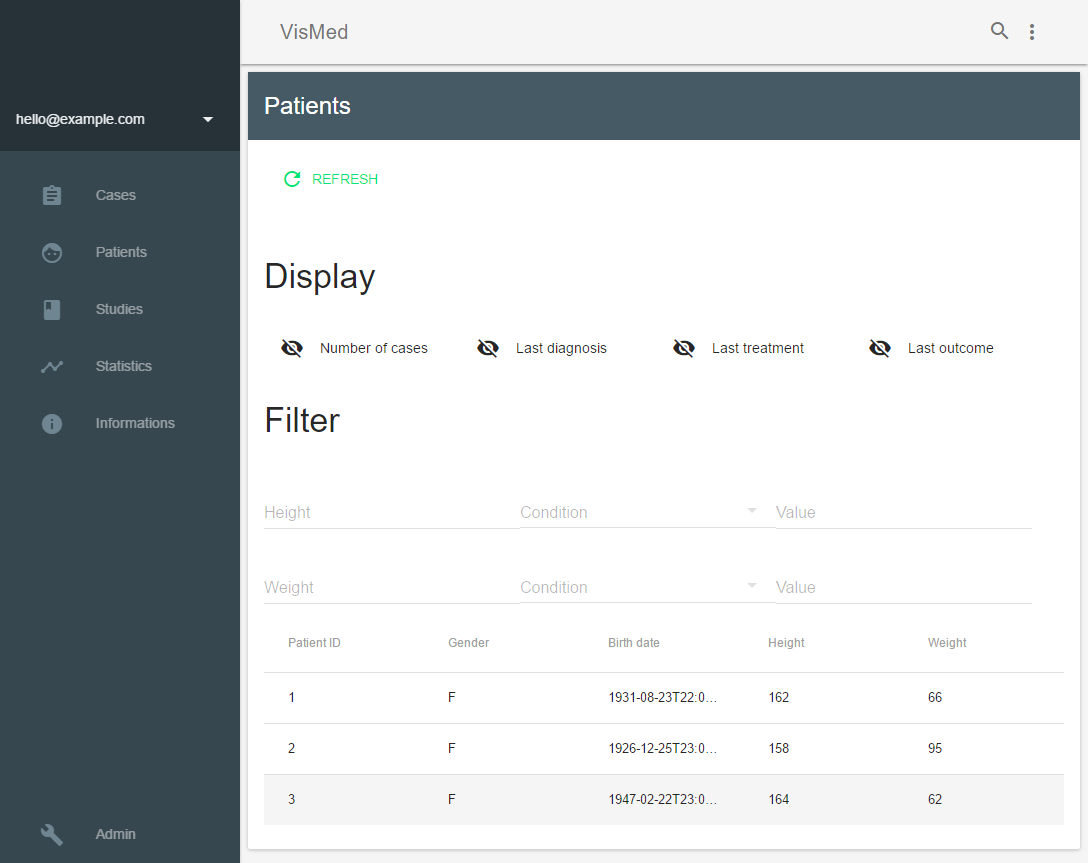
\includegraphics[width=1\textwidth]{images/realisation/proto1_2}
			\caption{Premier prototype de la page "Patients"}
			\label{proto1_2}
		\end{figure}

		On remarque que celle-ci reprend au mieux les éléments dessinés sur la maquette de la figure \ref{maquette_papier}. À nouveau, certains éléments ont été implémentés à l'aide de Material-UI, mais certains autres ont également dû être implémentés en utilisant directement le CSS de Material Design.

		Le principal élément de la page est un tableau présentant les données résumées de l'ensemble des patients. Ici, il s'agit de données d'exemple.

		Le but est ici de permettre deux actions différentes sur la liste des patients affichés : La partie "Display" permet d'afficher ou de cacher certaines colonnes, et la partie "Filter" permet. À noter que bien que l'interface soit implémentée ici, toutes les parties visibles ne sont pas encore fonctionnelles à ce stade. Les données affichées ne sont des données d'exemple, et les inputs de l'utilisateur (sur les parties Display et Filter) sont sans effet.

	\subsection{Communication des données}

		Une fois que le frontend est capable d'afficher des informations, il est encore nécessaire de le faire communiquer avec le serveur afin d'afficher les vraies données.

		\subsubsection{Flux de données}

			Comme nous utilisons et suivons le modèle Flux, il est nécessaire d'établir la logique du flux des données. Comme décrit dans le chapitre Analyse, Flux recommande l'utilisation d'un flux unidirectionnel des données.

			\begin{figure}[!ht]
				\centering
				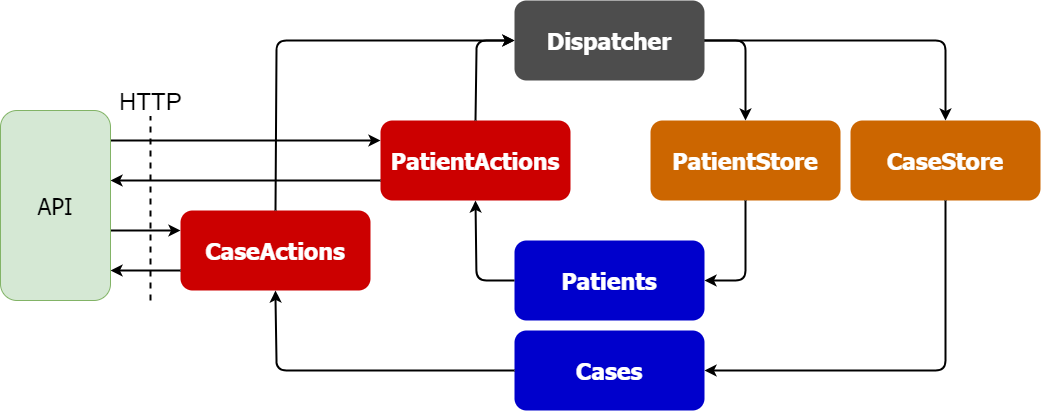
\includegraphics[width=1\textwidth]{images/realisation/vismedflux}
				\caption{Flux de données de l'application}
				\label{vismedflux}
			\end{figure}

			En suivant leurs recommandations, il a été possible d'établir le schéma illustré à la figure \ref{vismedflux}, montrant la manière dont les données sont échangées à travers de l'application React. On y voit les différents Classes et Composants qui interagissent dans l'échange de données :
			\begin{description}
				\item[\texttt{CaseActions} et \texttt{PatientActions}] Classes qui vont communiquer avec l'API du serveur lorsqu'on leur en fait la demande. Vont demander les données, et les transmettre au \texttt{Dispatcher} une fois reçues.
				\item[\texttt{Dispatcher}] Classe provenant de Flux, qui s'occupe de transmettre les données reçues aux Stores qui les stockent.
				\item[\texttt{PatientStore} et \texttt{CaseStore}]
				Classes qui stockent les données reçues depuis le \texttt{Dispatcher}. Elles servent à alimenter les vues \texttt{Patients} et \texttt{Cases} en données lorsqu'elles en ont besoin.
				\item[\texttt{Patients} et \texttt{Cases}] Composants React qui affichent respectivement la liste des patients, et la liste des cas. Chaque composant s'attache à son Store respectif, et affiche les données de celui-ci.
			\end{description}

			Au lancement de l'application, \texttt{PatientActions} et \texttt{CaseActions} agissent en demandant au serveur les données une première fois, ce qui va déclencher le reste de la boucle de réaction et ainsi pouvoir fournir des données aux composants \texttt{Patients} et \texttt{Cases} lorsque ceux-ci doivent être affichés.

\section{Implémentation backend}

	\subsection{Structure du backend}

		Pour la réalisation de la connexion entre la partie applicative métier et la partie base de données, il a été nécessaire de s'adapter à la structure hiérarchique des machines hébergeant l'application à l'EPFL. En effet, une contrainte est que le serveur hébergeant la base de données MySQL est accessible uniquement depuis l'intérieur du réseau.

		Bien que cela ne soit pas un problème pour l'application finale qui tournera sur un serveur de l'EPFL, cela complique la phase de développement durant laquelle il est nécessaire d'utiliser un autre serveur de l'EPFL comme proxy pour s'y connecter.

		\begin{figure}[h]
			\centering
			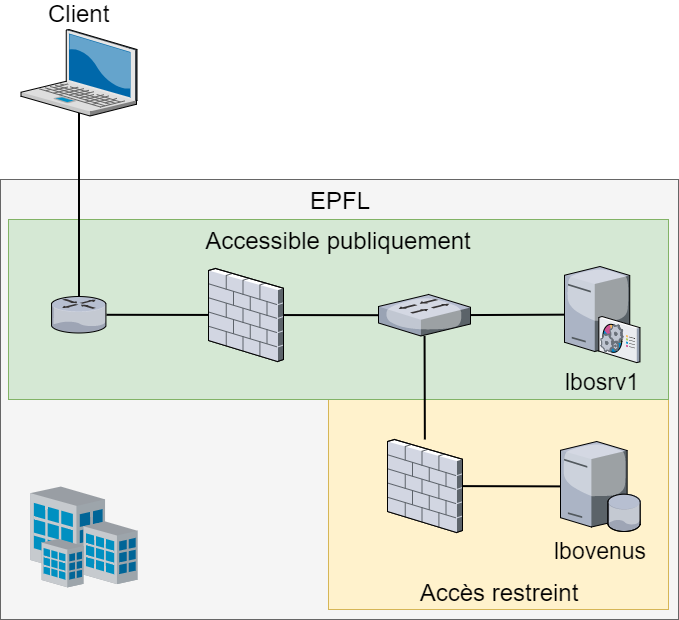
\includegraphics[width=1\textwidth]{images/realisation/Schema_EPFL}
			\caption{Schéma de l'architecture réseau de l'EPFL utilisée par VisMed}
			\label{schema-epfl}
		\end{figure}

		La figure~\ref{schema-epfl} montre, parmi l'architecture de l'EPFL traversée, les deux serveurs utilisés par l'installation de VisMed. On y voit :
		\begin{description}
			\item[lbosrv1] Il s'agit du serveur "principal", sur lequel tourne le code backend de l'application. Il s'agit également du serveur qui va écouter le port 80, et donc recevoir les requêtes HTTP de clients externes et y répondre. Mais afin de pouvoir faire son travail correctement, il aura généralement besoin d'accéder à des données se trouvant sur la base de données des cas et des patients. Celle-ci se trouve sur le deuxième serveur utilisé, qui se nomme \texttt{lbovenus}.
			\item[lbovenus] Il s'agit du serveur contenant la base de données médicales actuelle. Celle-ci, de type MySQL, contient les données concernant les patients de l'hôpital, ainsi que leurs cas. Cette base de données se trouve derrière un pare-feu supplémentaire, et est inaccessible depuis l'extérieur de l'EPFL. Le seul moyen de pouvoir la questionner est d'être à l'intérieur du réseau de l'EPFL, où se trouve également \texttt{lbosrv1}. C'est pourquoi il y a accès sans problème.
		\end{description}

	\subsection{Express.js}

		La logique du serveur a été développée en utilisant node.js ainsi que la librairie Express. Express s'occupe d'écouter sur un port particulier et de répondre aux requêtes avec les informations adéquates. Dans notre cas, le port utilisé est le \texttt{3000}. Elle sert les quelques ressources statiques nécessaires (script JavaScript dont l'application compilée, mais également les fichiers CSS). Mais également, elle répond aux requêtes sur l'API définie.

		Les requêtes possibles de l'API sont peu nombreuses :

		\begin{description}
			\item[\texttt{GET /api/patients}] Renvoie la liste complète des patients ainsi que toutes leurs informations.
			\item[\texttt{GET /api/cases}] Renvoie la liste complète des patients ainsi que toutes leurs informations.
		\end{description}

		Pour fournir les informations nécessaires lors de l'appel à l'un de ces deux méthodes, l'application se connecte à la base de données, effectue une requête sur la vue correspondante, et formate le résultat pour l'envoyer en JSON au client.

	\subsection{Base de données}

		Pour simplifier la sélection des données utiles à partir de la structure initiale de la base de données, des vues SQL ont été ajoutées.
		Les deux vues, \texttt{case\_view\_all} et \texttt{patient\_view\_all}, joignent toutes les données nécessaires de plusieurs tables afin de constituer la réponse voulue aux requêtes sur les deux méthodes de l'API précédemment décrites.

\section{Evaluation}

	\subsection{Heuristique et adaptations}

		Ce prototype a été discuté à de nombreuses reprises.
		Des évaluations ont été faites de semaine en semaine, et ont mené à de nombreuses améliorations basées sur des critères ergonomiques.

		Durant ces séances d'évaluation heuristique, beaucoup de points discutés ont été à adapter afin de proposer une interface avec une meilleure ergonomie. Les modifications qui en résultent suivent les critères ergonomiques de Bastien et Scapin\cite{ergoweb} tels que la cohérence, la lisibilité ou le principe du groupement/distinction. Par exemple, sur la page Patients, on peut noter :

		\begin{itemize}
			\item Augmentation de la taille de police
			\item Retrait des titres "Display" et "Filter"
			\item Elargissement de la zone d'affichage à toute la largeur de la page
			\item Utilisation du Header pour y placer les filtres de display
			\item Retrait du bouton d'actualisation
			\item Augmentation de la visibilité des titres de colonne
		\end{itemize}

		De même, des changements plus généraux ont été appliqués :

		\begin{itemize}
			\item Augmentation de la taille de police des liens
			\item Augmentation du contraste de la police et des icônes des liens
			\item Retrait du titre "VisMed" dans le Header
			\item Passage du bouton "Admin" en haut du Drawer, avec les autres liens
			\item Surbrillance du lien actuellement sélectionné
		\end{itemize}

		Les évaluations heuristiques ont donc permis au prototype d'évoluer à la fois en termes de fonctionnalités grâce au contact avec le client, et à la fois utilisabilité grâce aux critères d'ergonomie qui ont été appliqués. Les adaptations se sont fait itérativement sur plusieurs semaines, et ont mené à la production d'un deuxième prototype. 

	\subsection{Validation par les clients}

		Les prototypes ont été montrés au client à plusieurs reprises afin de bénéficier d'un feedback, en plus de la première réunion en personne avec tous les intervenants. La confirmation de celui-ci de la direction du développement nous a permis de s'assurer que le projet allait dans le sens demandé.
\chapter{Prototype 2}
%%%%%%%%%%%%%%%%%%%%%%%%%%
%                          %
% ----- INTRODUCTION ----- %
%                          %
%%%%%%%%%%%%%%%%%%%%%%%%%%

\section{Fonctionnalités}

	La deuxième itération de l'application vise à couvrir certaines autres fonctionnalités :
	\begin{itemize}
		\item Recherche d'informations dans la page "Cases" et "Patients"
		\item Page d'édition d'un "Case"
		\item Page d'édition d'un "Patient"
	\end{itemize}

\section{Conception}

	Le deuxième prototype de l'application comprend donc des nouveautés en termes de fonctionnalités. En effet, après avoir déployé et présenté le premier prototypes, des remarques de la part du client ont centré le développement sur les deux fonctionnalités suivantes les plus intéressantes; la recherche d'informations, et l'édition de données. La fonctionnalité principale est l'édition des données, et il fallait pouvoir éditer la plupart des données affichées : Aussi bien celles d'un cas que celles d'un patient.

	\section{Pages d'édition}
	
		Deux nouvelles pages sont donc consacrées à afficher et permettre la modification d'une part d'un cas, et d'autre part d'un patient. Ces pages sont accessibles en cliquant respectivement sur la ligne d'un, ou sur la ligne d'un patient dans la liste. Cette page affiche toutes les informations relatives au cas ou au patient concerné, mais chacune a une spécificité supplémentaire :

		\begin{itemize}
			\item La page "Case" affiche également les informations du Patient concerné, ainsi qu'un bouton "Edit" redirigeant l'utilisateur vers la page d'édition du Patient.
			\item Le page "Patient" affiche l'ensemble des cas qui concernent ce patient. Cliquer sur un cas dirige l'utilisateur vers la page d'édition de celui-ci.
		\end{itemize}

		La figure \ref{proto2_1} montre un prototype de la page de modification d'un cas.

		\begin{figure}[!h]
			\centering
			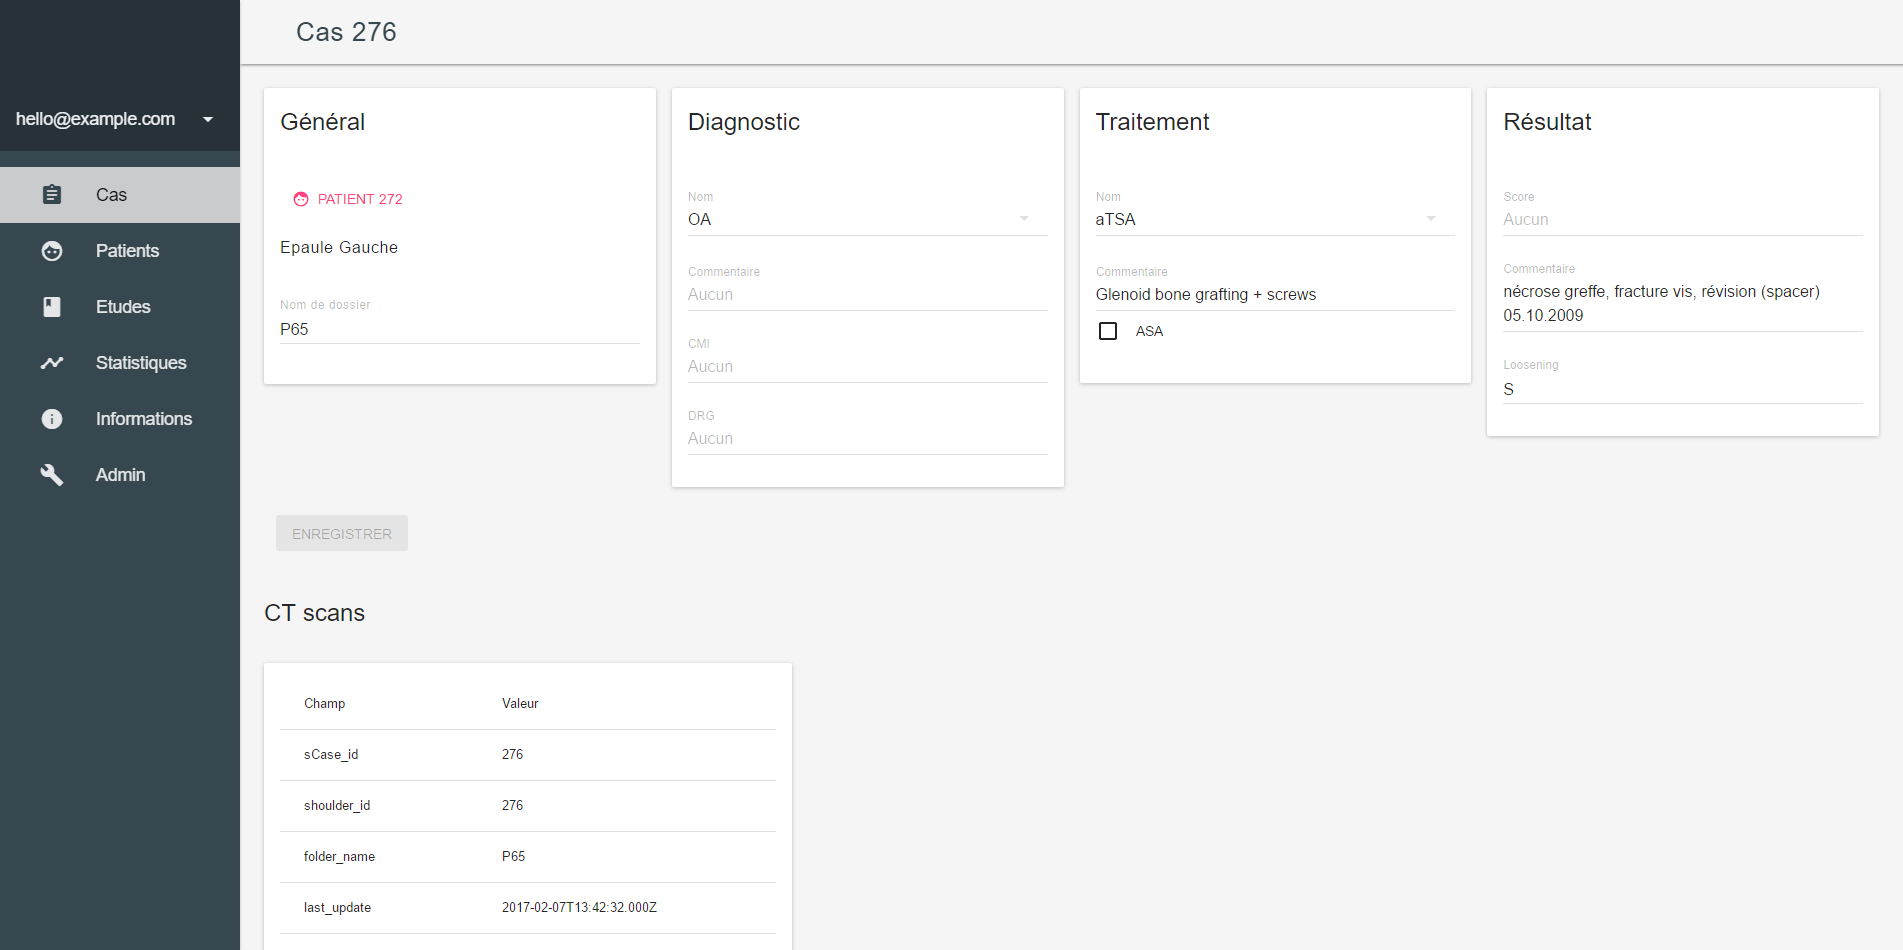
\includegraphics[width=1\textwidth]{images/realisation/proto2_1}
			\caption{Prototype de la page de modification d'un cas}
			\label{proto2_1}
		\end{figure}

	\section{Recherche}

		Une autre fonctionnalité a été modifiée : Le filtrage des données. Le système initial de filtres a été changé en un champ de recherche, qui est plus facile et plus rapide à utiliser. Ce filtre sera présent aussi bien sur la page Cases que sur la page Patients. Ecrire dans le champ recherche la chaîne de caractères entrée dans l'ensemble des champs des données affichées.
		La figure \ref{proto2_2} montre un prototype de la page de la liste des cas.

		\begin{figure}[!h]
			\centering
			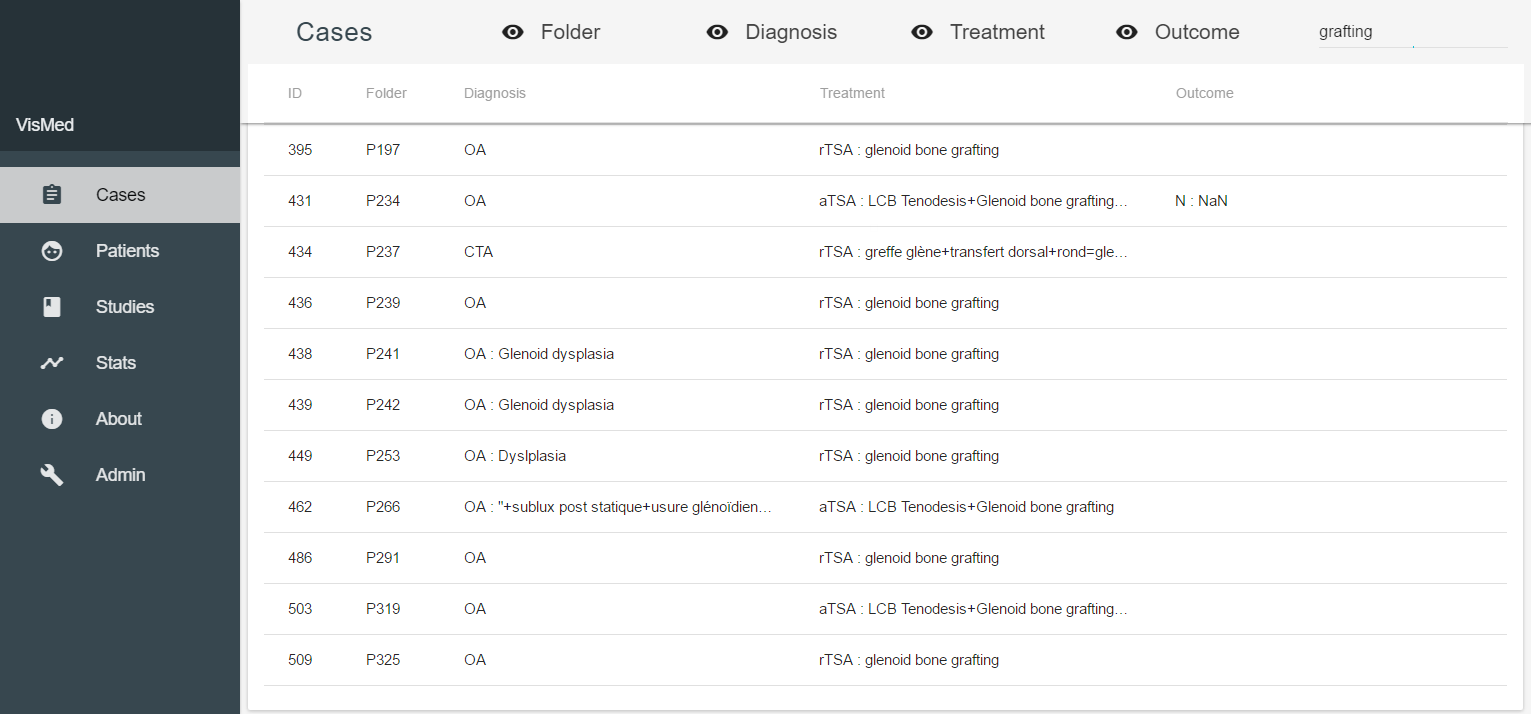
\includegraphics[width=1\textwidth]{images/realisation/proto2_2}
			\caption{Prototype de la liste des cas avec recherche de mot clé}
			\label{proto2_2}
		\end{figure}


\section{Implémentation}

	\subsection{Pages d'édition}

		L'implémentation des pages d'édition d'un cas et d'un patient s'est naturellement faite pas l'addition de deux nouveaux composants \texttt{Case} et \texttt{Patient}.

		\subsubsection{Case}

			Les données à afficher sur la page de Cas sont plus larges que les données affichées sur la liste des cas : En effet, il est nécessaire ici de montrer la liste des CT scans liés à un cas. Cet ajout a nécessité des modifications dans le backend : L'ajout d'un endpoint destiné à renvoyer non seulement toutes les informations d'un cas, mais également l'ensemble des informations des CT liés à ce cas.

			La méthode suivante a donc été ajoutée au serveur :
			\begin{description}
				\item[\texttt{GET /api/case/<id>}] Renvoie les informations du cas \texttt{<id>} ainsi que les CT qui sont liées
			\end{description}

			Celle-ci fait appel à une vue SQL implémentée sous le nom de \texttt{ct\_view}.

			De plus, la possibilité de modifier les données du cas a également nécessité tout d'abord l'ajout d'une méthode sur le serveur :

			\begin{description}
				\item[\texttt{POST /api/case/<id>}] Modifie les informations du cas \texttt{<id>}
			\end{description}

			Cette méthode fait appel à une procédure stockée SQL implémentée pour cette fonctionnalité. Nommée \texttt{updateCase}, elle prend en paramètre l'ensemble des données modifiables d'un cas. Si un paramètre est laissé vide (C'est le cas lorsqu'il n'est pas modifié par l'utilisateur dans l'interface), il est ignoré et n'est pas mis à jour. Ceci a été fait pour éviter le cas où plusieurs modifications concurrentes pourraient écraser des nouvelles données avec des données non mises à jour.

			Afin de repérer facilement quelles données vont être mises à jour, les champs modifiés dans l'interface sont également mis en surbrillance avec une couleur bleue. La figure montre un champ "Commentaire" modifié, qui se distingue des autres champs de sa catégorie.

			\begin{figure}[!h]
				\centering
				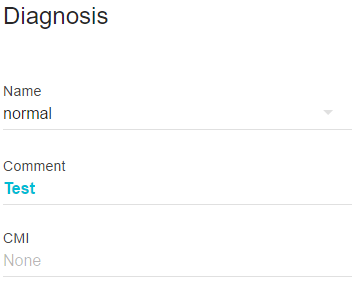
\includegraphics[width=0.4\textwidth]{images/realisation/proto2_3}
				\caption{Mise en évidence du champ modifié}
				\label{proto2_3}
			\end{figure}

		\subsubsection{Patient}

			L'ajout de la page de modification d'un Patient a demandé des efforts semblables à ceux de la page Case. On retrouve donc l'ajout de deux nouvelles méthodes à l'API, cette fois-ci pour un patient :

			\begin{description}
				\item[\texttt{GET /api/patient/<id>}] Renvoie les informations du patient \texttt{<id>} ainsi que des cas qui lui sont liées
				\item[\texttt{POST /api/patient/<id>}] Modifie les informations du patient \texttt{<id>}
			\end{description}

			Une des différences est que la méthode \texttt{GET /api/patient/<id>} renvoie également la liste des cas appartenant à un patient.

			De même, une procédure stockée SQL a également été implémentée pour permettre la modification facile des données d'un Patient, sous le nom de \texttt{updatePatient}.

	\subsection{Recherche}

		L'implémentation du champ de recherche ainsi que les boutons d'affichage des colonnes dans le \texttt{Header} a nécessité la création de composants spécialisées pour gérer ce type de Header, en dehors des Headers classiques. Les composants \texttt{CasesHeader} et \texttt{PatientsHeader} ont été crées, et affichent donc les contrôles nécessaires pour afficher ou cacher des colonnes, ainsi que gérer la recherche.

		Ces deux composants doivent communiquer avec les composants \texttt{Cases} et \texttt{Patients} de base. Il a donc été nécessaire de faire passer cette communication par le flux d'informations installé jusqu'ici.

		Lorsque l'utilisateur modifie l'affichage de colonnes ou la recherche appliqué, une action est donc crée et dispatchée sur le Store correspondant (soit CaseStore, soit PatientStore). La vue de la liste est ensuite mise à jour à partir des informations du store. Cependant, contrairement à précédemment, toute ces opérations se sont du côté client, et aucune communication avec le serveur n'est requise.

\section{Evaluation heuristique et adaptations}

	Au cours du développement de cette application, plusieurs évaluations formatives ont été réalisées. Chaque évaluation se focalise sur une ou plusieurs parties de l'application différentes, mais le but est généralement commun : On souhaite faire le point sur l'état actuel de l'utilisabilité de l'application en prenant un point de vue utilisateur, et en se posant des questions sur le design actuel de l'interface.

	Bien que fonctionnelle, ces vues n'étaient pas optimales sur le plan ergonomique. Une évaluation formative a montré plusieurs points à changer :
	\begin{itemize}
		\item La première information affichée sur la page Cas concerne le Patient : Cela est inadéquat
		\item Le bouton "Save" ne devrait concerner que la partie de la page effectivement modifiable
		\item Les champs d'input contiennent un label trop peu visible : Il est nécessaire d'améliorer leur visibilité
		\item Le champ de date est présent dans la base de données, mais pas sur la page : Il faut l'ajouter
	\end{itemize}

	Ces dernières remarques ont donc été prises en compte afin de réaliser la dernière version de l'interface de l'application.

\section{Résultat}

	L'application est fonctionnelle, et propose les éléments suivants :

	Les figures~\ref{cases1}, \ref{cases2} montrent respectivement la vue de la page de l'ensemble des Cas, ainsi que la vue de la page d'un Cas spécifique.

	\begin{figure}[!h]
		\centering
		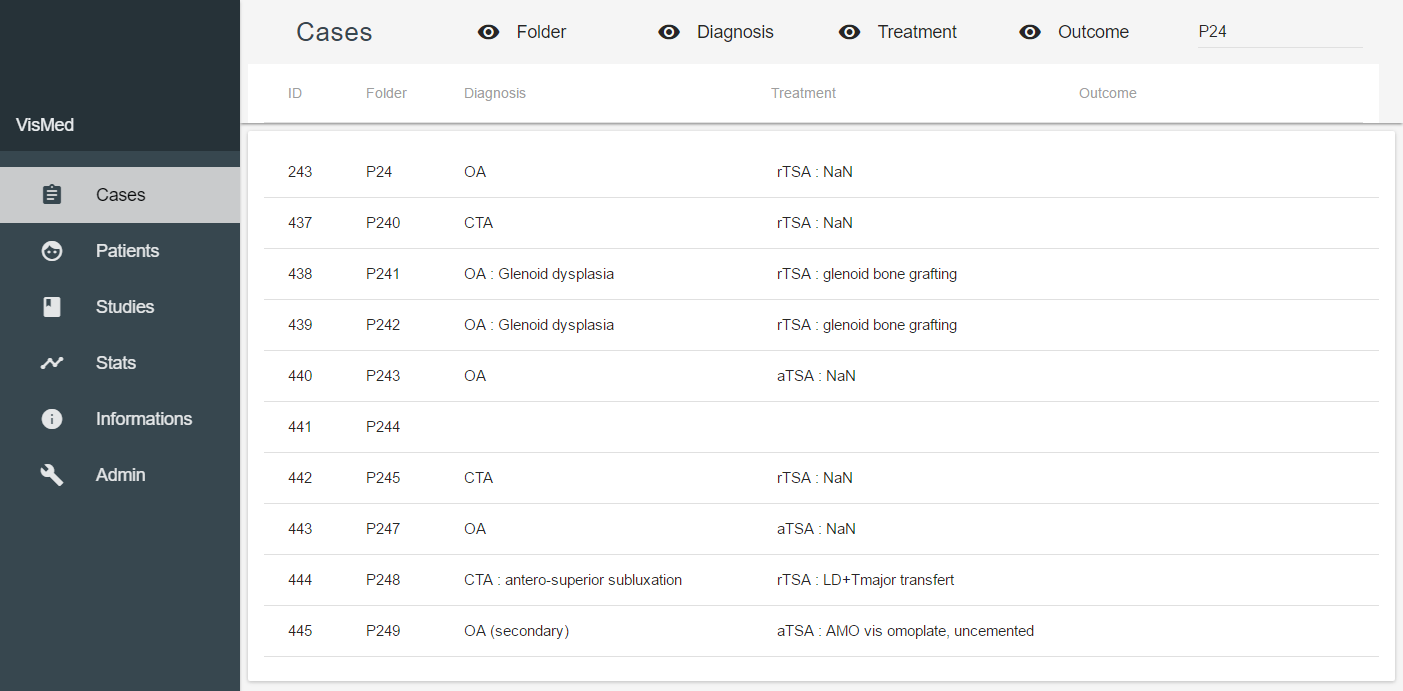
\includegraphics[width=1\textwidth]{images/realisation/cases1}
		\caption{Page "Cases" mise à jour, montrant la recherche de l'information 'P24'}
		\label{cases1}
	\end{figure}

	\begin{figure}[!h]
		\centering
		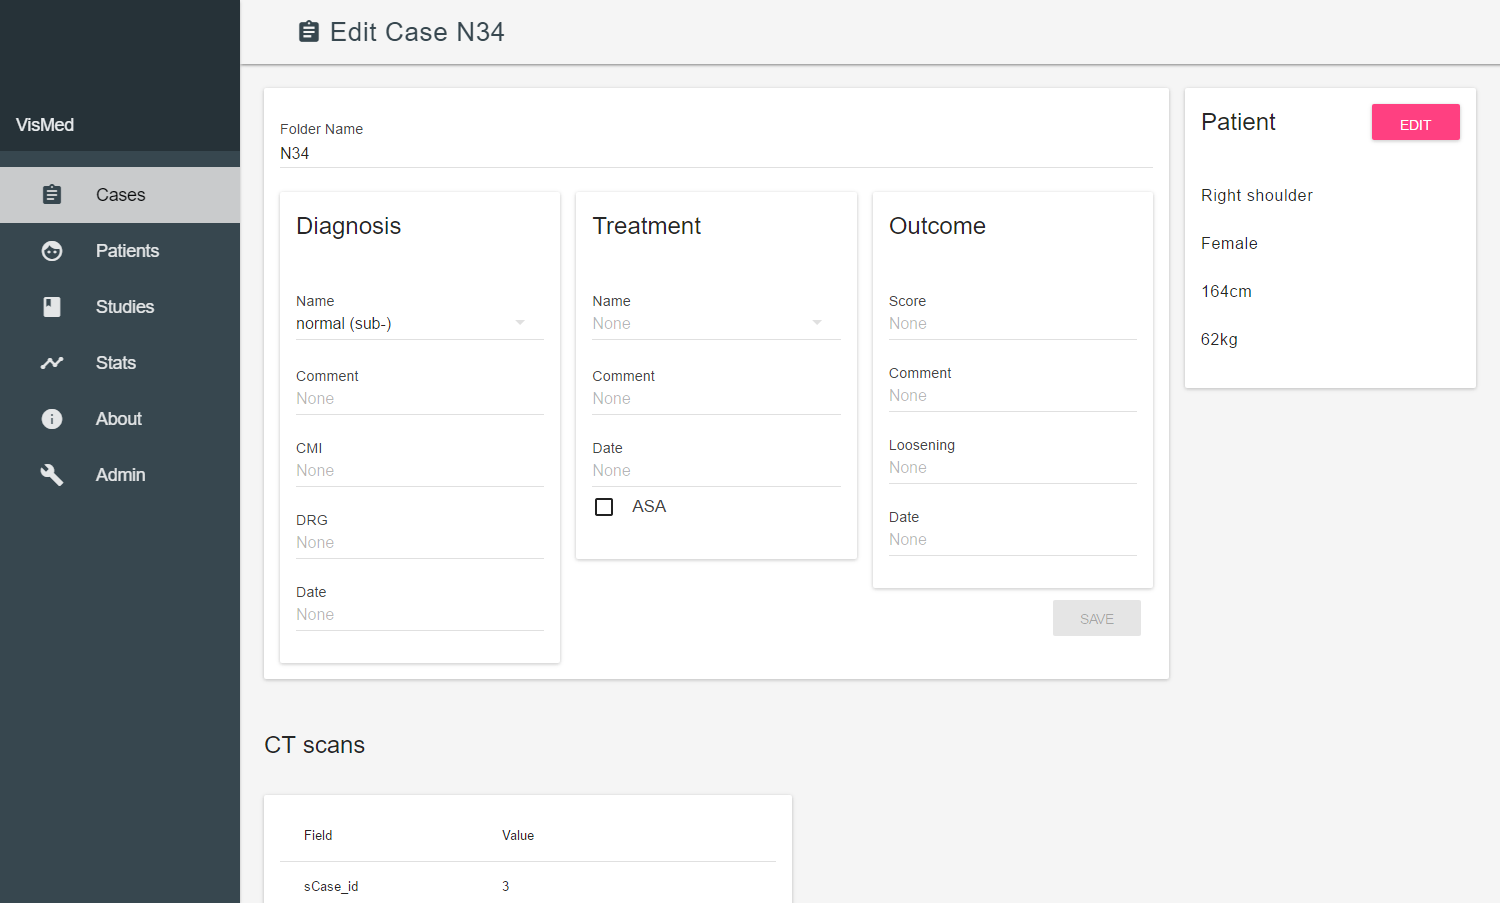
\includegraphics[width=1\textwidth]{images/realisation/cases2}
		\caption{Page finale d'édition d'un cas}
		\label{cases2}
	\end{figure}

	Les figures~\ref{patients1}, \ref{patients2} montrent respectivement la vue de la page de l'ensemble des Patients, ainsi que la vue de la page d'un Patient spécifique.

	\begin{figure}[!h]
		\centering
		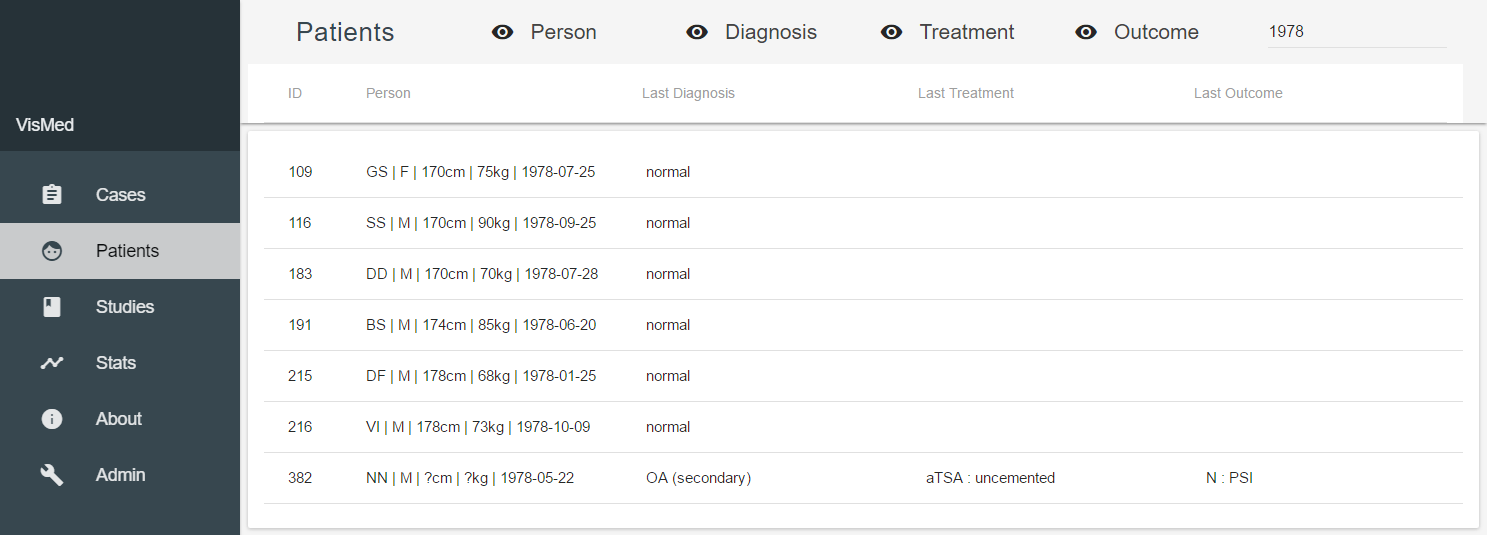
\includegraphics[width=1\textwidth]{images/realisation/patients1}
		\caption{Page "Patients" mise à jour, montrant la recherche de l'information '1980'}
		\label{patients1}
	\end{figure}

	\begin{figure}[!h]
		\centering
		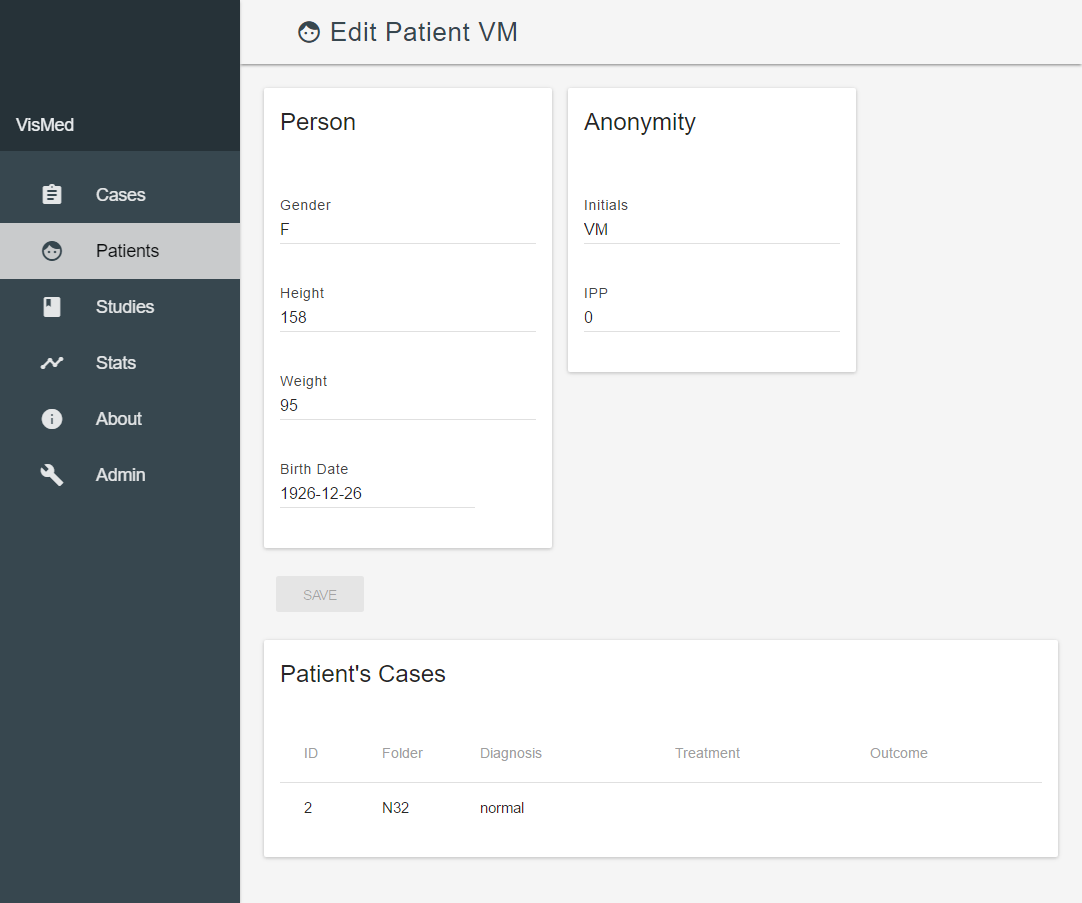
\includegraphics[width=1\textwidth]{images/realisation/patients2}
		\caption{Page finale d'édition d'un patient}
		\label{patients2}
	\end{figure}

\chapter{Conclusion}
%%%%%%%%%%%%%%%%%%%%%%%%%%%%%%
%                               %
% ----- CONCLUSION PROJET ----- %
%                               %
%%%%%%%%%%%%%%%%%%%%%%%%%%%%%%

\section{Conclusion du projet}

	\subsection{Délivrables}

		Ce projet est passé par plusieurs étapes distinctes qui ont mené à la production de plusieurs délivrables :
		\begin{itemize}
			\item Analyse des besoins
			\item Analyse des technologies
			\item Maquette papier
			\item Premier prototype : Développement et évaluation
			\item Deuxième prototype : Développement et évaluation
			\item Application finale
		\end{itemize}
		Chacune de ces étapes nous a amené à produire une itération supplémentaire contenant à la fois des nouveautés fonctionnelles, mais aussi des changements et améliorations ergonomiques. Chaque itération nous a donc rapproché du produit final.

	\subsection{Conclusion générale}

		Bien que le scope intial du projet soit surdimensionné, nous avons pu communiquer avec le client afin de clarifier quelles étaient les attentes principales. Les fonctionnalités centrales ont donc été implémentées, et le produit final répond donc aux besoins les plus importants du client. Ainsi, l'application finale permet de :
		\begin{itemize}
			\item Afficher des informations de l'ensemble des cas
			\item Rechercher des informations parmi les cas
			\item Afficher et modifier les données d'un cas particulier
			\item Afficher des informations de l'ensemble des patients
			\item Rechercher des informations parmi les patients
			\item Afficher et modifier les données d'un patient particulier
		\end{itemize}
		

	\subsection{Perspectives}

		Le projet dans son état final contient plusieurs pages non implémentées :

		\begin{itemize}
			\item Studies
			\item Stats
			\item Admin
		\end{itemize}

		Ces pages sont actuellement vides et un projet futur pourrait commencer par y ajouter du contenu, après avoir défini clairement leur utilité.

		De plus, l'application dans son ensemble pourrait bénéficier d'un véritable système de login, ainsi que d'une sécurité accrue, notamment dans les accès aux méthodes de l'API.

%%%%%%%%%%%%%%%%%%%%%%%%%%%%%%%%%%%
%                                    %
% ----- CONCLUSION PERSONNELLE ----- %
%                                    %
%%%%%%%%%%%%%%%%%%%%%%%%%%%%%%%%%%%

\section{Conclusion personnelle}

	J'ai beaucoup apprécié travailler sur ce projet pour deux raisons différentes :

	Tout d'abord, j'ai pu voir et gérer un processus centré sur l'utilisateur. Cette approche itérative change de ce que j'ai eu l'habitude de faire, et m'a permis de découvrir une autre manière de produire un résultat.

	Et également, j'ai pu me familiariser et utiliser dans une situation pratique certaines des dernières technologies du monde du Web. Bien que toutes les librairies ne m'aient pas plu (J'ai trouvé Material-UI assez lacunaire), j'ai beaucoup aimé travailler avec React et Flux, qui ont l'air assez matures pour pouvoir produire des interfaces de qualité et maintenables.
	

\begin{thebibliography}{9}

\bibitem{react}
  Facebook Inc.,
  \emph{A JavaScript library for building user interfaces - React},
  \url{https://facebook.github.io/react},
  Consulté en ligne en Mars 2017,
  2017.

\bibitem{valuecoders-choosereact}
  ValueCoders,
  \emph{5 reasons to choose Facebook’s ReactJS},
  \url{http://www.valuecoders.com/blog/technology-and-apps/5-reasons-choose-facebooks-reactjs/},
  Consulté en ligne en Avril 2017,
  2017.

\bibitem{nodejs}
  Node.js,
  \emph{Node.js},
  \url{https://nodejs.org},
  Consulté en ligne en Avril 2017,
  2017.

\bibitem{npm}
  npm,
  \emph{npm},
  \url{https://npmjs.com},
  Consulté en ligne en Avril 2017,
  2017.

\bibitem{webpack}
  webpack,
  \emph{webpack},
  \url{https://webpack.github.io/docs/},
  Consulté en ligne en Avril 2017,
  2017.

\bibitem{material-ui}
  Material-UI,
  \emph{Material-UI},
  \url{http://www.material-ui.com},
  Consulté en ligne en Avril 2017,
  2017.

\bibitem{express}
  Express,
  \emph{Express - Infrastructure d'application Web Node.js},
  \url{http://expressjs.com/fr/},
  Consulté en ligne en Avril 2017,
  2017.

\bibitem{mysql}
  MySQL,
  \emph{MySQL},
  \url{https://www.mysql.fr/},
  Consulté en ligne en Avril 2017,
  2017.

\bibitem{material-design-guidelines}
  Material Design,
  \emph{Introduction - Material Design - Material design guidelines},
  \url{https://material.io/guidelines/},
  Consulté en ligne en Avril 2017,
  2017.

\bibitem{jsx}
  React,
  \emph{JSX in Depth},
  \url{https://facebook.github.io/react/docs/jsx-in-depth.html},
  Consulté en ligne en Avril 2017,
  2017.

\bibitem{tutorial-react}
  React,
  \emph{Tutorial: Intro to React},
  \url{https://facebook.github.io/react/tutorial/tutorial.html},
  Consulté en ligne en Avril 2017,
  2017.

\bibitem{flux}
  Facebook Inc.,
  \emph{Flux | Application Architecture for Building User Interfaces},
  \url{https://facebook.github.io/flux/},
  Consulté en ligne en Mai 2017,
  2017.

\bibitem{flux-github}
  GitHub Inc.,
  \emph{facebook/flux: Application Architecture for Building User Interfaces},
  \url{https://github.com/facebook/flux},
  Consulté en ligne en Mai 2017,
  2017.

\bibitem{learncode-academy}
  YouTube,
  \emph{React JS Tutorials},
  \url{https://www.youtube.com/playlist?list=PLoYCgNOIyGABj2GQSlDRjgvXtqfDxKm5b},
  Consulté en ligne en Mars 2017,
  2017.

\bibitem{react-boilerplate}
  GitHub Inc.,
  \emph{Spartano/LearnCode.academy-REACT-JS-TUTORIAL},
  \url{https://github.com/Spartano/LearnCode.academy-REACT-JS-TUTORIAL},
  Consulté en ligne en Mars 2017,
  2017.

\bibitem{materialui-drawer}
  Material UI,
  \emph{Drawer},
  \url{http://www.material-ui.com/#/components/drawer},
  Consulté en ligne en Mars 2017,
  2017.

\bibitem{react-router}
  React Training,
  \emph{React Router: Declarative Routing for React.js},
  \url{https://reacttraining.com/react-router},
  Consulté en ligne en Avril 2017,
  2017.

\bibitem{ergoweb}
  Ergoweb,
  \emph{Critères ergonomique de Bastien et Scapin},
  \url{http://ergoweb.ca/criteres/},
  Consulté en ligne en Juin 2017,
  2017.

\end{thebibliography}

\printglossary

\chapter*{Remerciements}
Je tiens à remercier ma superviseure Sandy Ingram pour m'avoir guidé lors des décisions à prendre, ainsi que m'avoir soutenu et aidé tout au long de ce projet.

\chapter*{Déclaration d'honneur}
Je, soussigné, Kewin Dousse, déclare sur l’honneur que le travail rendu est le fruit d’un travail personnel. Je certifie ne pas avoir eu recours au plagiat ou à toutes autres formes de fraudes. Toutes les sources d’information utilisées et les citations d’auteur ont été clairement mentionnées.

\bigskip
\bigskip

Lieu \hfil Date \hfil Signature

\appendix

\chapter{Historique des versions}
Voici l’historique des versions de ce document.

\begin{itemize}
	\item 0.1 : Template du document
	\item 0.2 : Chapitre "Analyse"
	\item 0.3 : Correction, complétion du chapitre "Analyse", rédaction d'une partie du chapitre "Conception"
	\item 0.4 : Rédaction de la plupart de la partie "Design du système", anciennement "Conception"
	\item 0.5 : Rédaction de la partie "Développement des vues"
	\item 0.6 : Complétion du "Développement des Vues", réorganisation de la structure de parties précédentes, et début de la partie "Résultats"
	\item 0.7 : Fin de la rédaction du texte du rapport
	\item 1.0 : Correction, complétion du chapitre "Analyse", ajout des annexes
\end{itemize}

\chapter{Cahier des charges}
\section{Activités}

Le développement du projet peut se découper en plusieurs phases, qui elles-mêmes se divisent en plusieurs activités. Voici la liste de ces activités :

\begin{enumerate}
	\item Analyse des besoins
	\begin{enumerate}
		\item Analyse des features demandées
		\item Etude des cas d’utilisation
		\item Etude de la faisabilité des demandes
		\item Analyse de la correspondance avec la base de données existante
	\end{enumerate}
	\item Analyse des technologies
	\begin{enumerate}
		\item Analyse et choix des technologies pertinentes
		\item Apprentissage des technologies choisies
	\end{enumerate}
	\item Conception de l’application
	\begin{enumerate}
		\item Design de l’architecture générale de l’application
		\item Design de l’interaction et de la structure de navigation
		\item Prototypage
	\end{enumerate}
	\item Réalisation de l’application
	\begin{enumerate}
		\item Réalisation du code backend
		\item Réalisation du code frontend
		\item Evaluation du comportement fonctionnel de l’application
		\item Evaluation de la robustesse de l’application
	\end{enumerate}
	\item Evaluation itérative
	\begin{enumerate}
		\item Evaluation formative
		\item Evaluation sommative informelle et empirique
		\item Rétrospective du développement
	\end{enumerate}
\end{enumerate}

\section{Planification}
Le projet comporte une série de dates-clé qu’il est important de respecter :
\begin{center}
   \begin{tabular}{ | l | c | r | }
     \hline
		Date & Semaine & Tâche \\ \hline
		\color{red}Lundi 20 février 2017 & Semaine P1 & Début du projet \\ \hline
		Lundi 31 mars 2017 & Semaine P6 & Fin de l’apprentissage des technologies choisies \\ \hline
		Lundi 20 mai 2017 & Semaine P12 & Fin de l’implémentation de l’application \\ \hline
		\color{red}Vendredi 9 juin 2017 & Semaine P15 & Dépôt du rapport \\ \hline
		\color{red}19-30 juin 2017 & - & Défense orale \\ \hline
     \hline
   \end{tabular}
\end{center}

Les dates en rouge sont des dates de rendu officielles.
Les autres représentent des jalons dans l’avancement du projet.

\section{Diagramme de Gantt}
	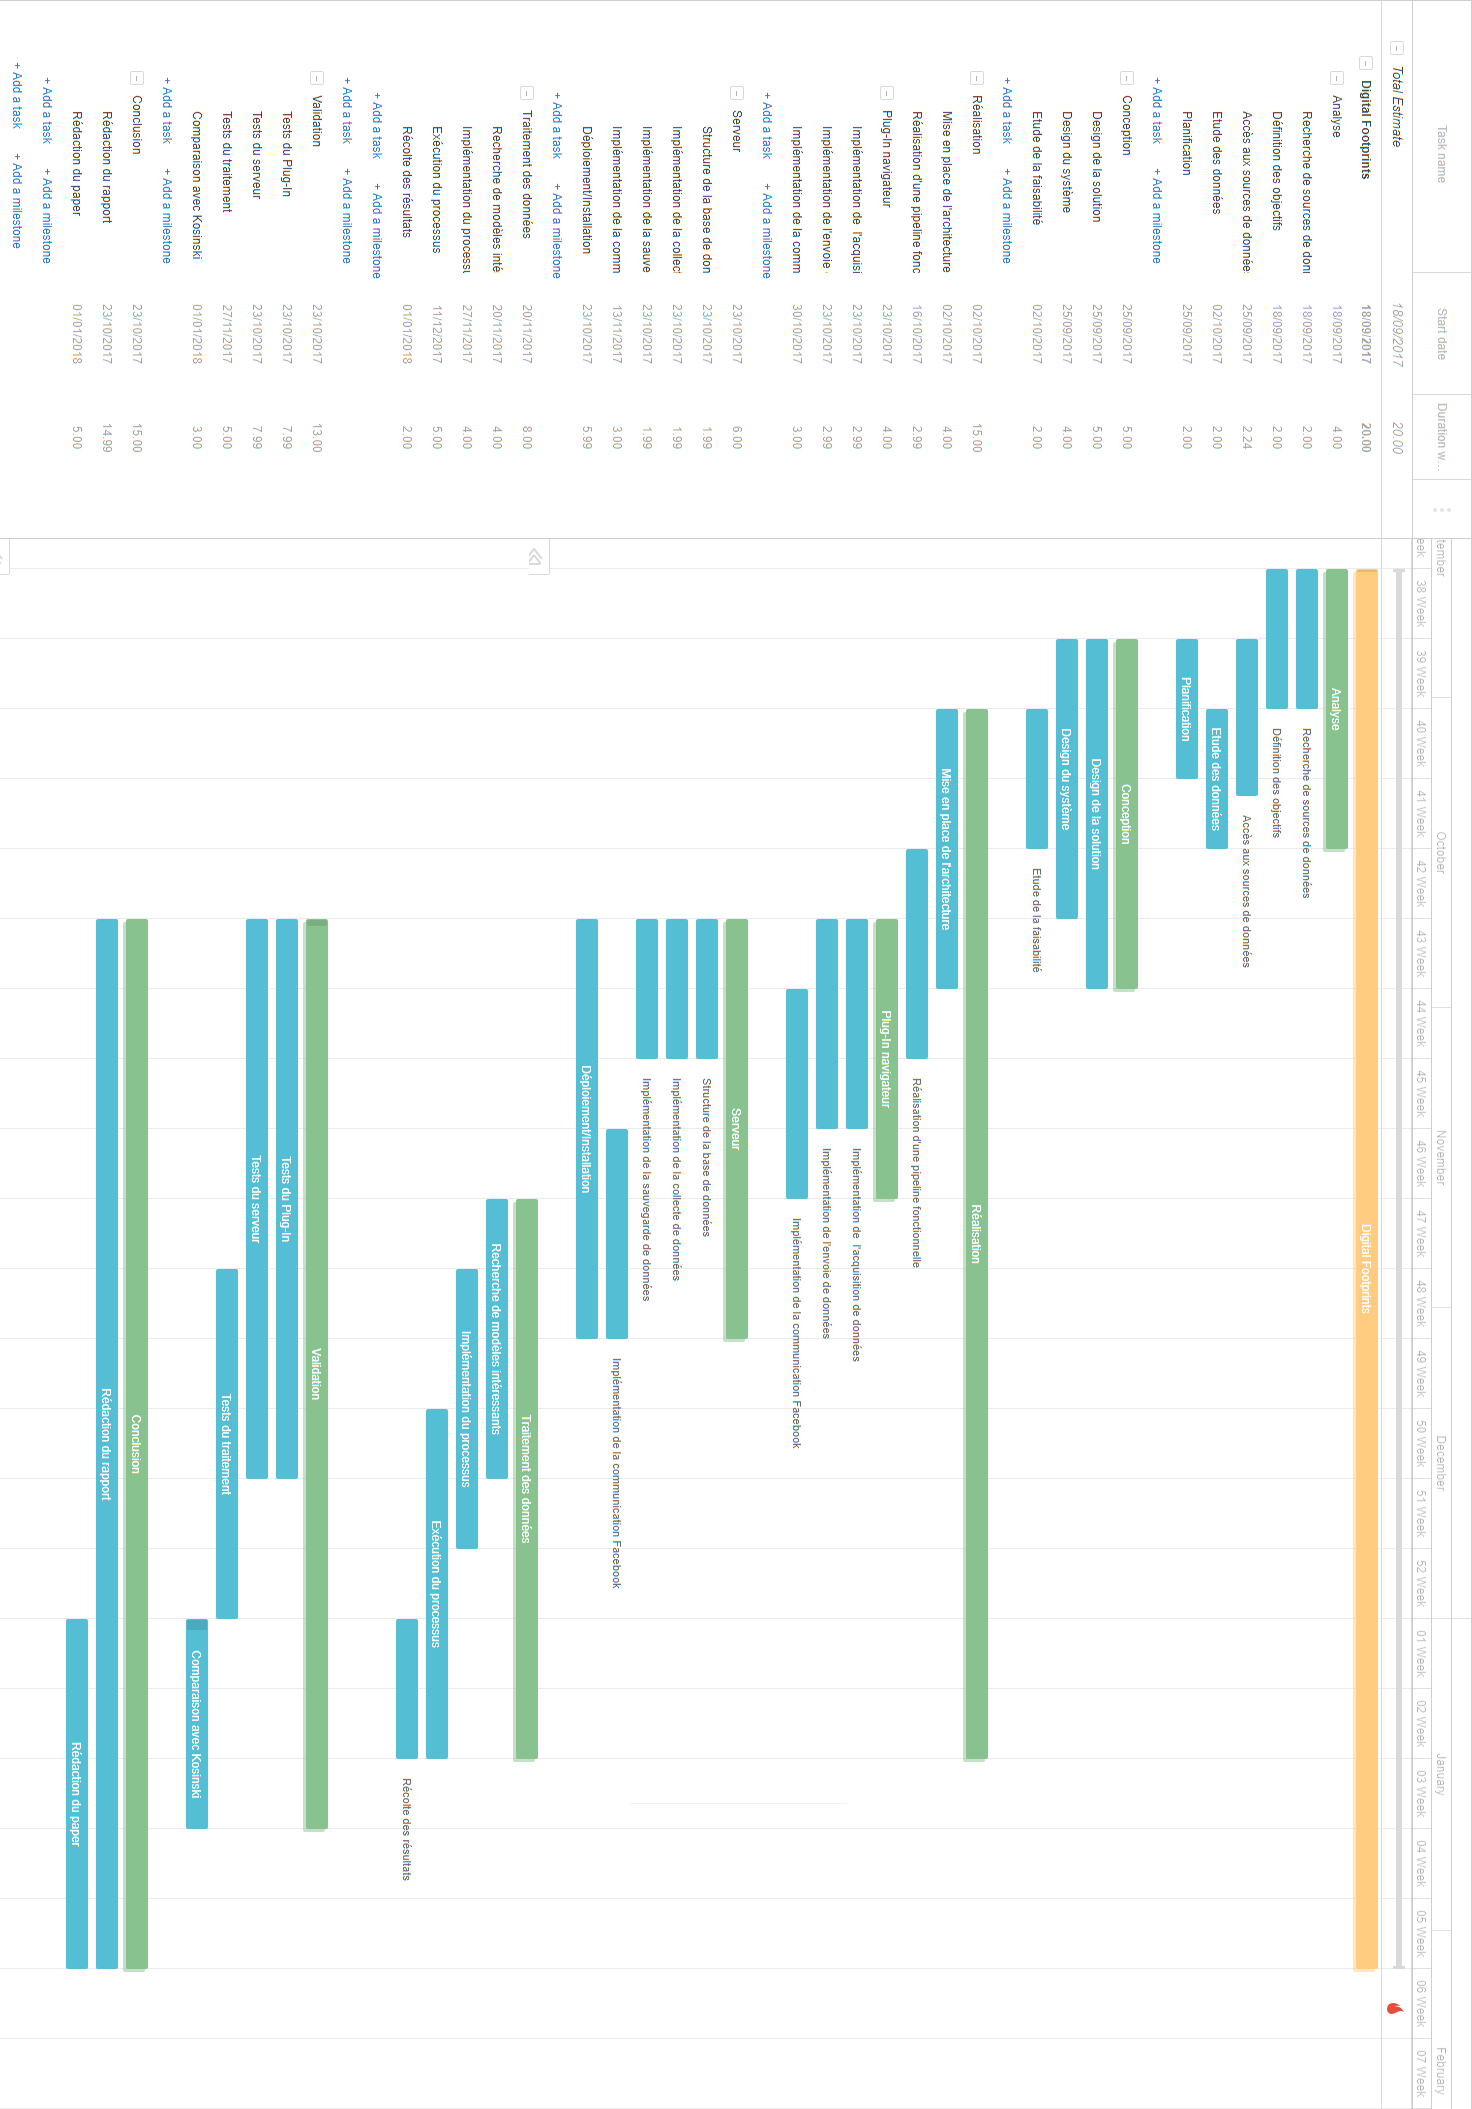
\includegraphics[width=0.51\textwidth]{images/annexes/cdc/gantt}

\chapter{Documentation}
\section{Localisation}

	L’ensemble des documents du projet est disponible à l’adresse suivante :
	\url{soon}

\section{Contenu}

	\subsection{GitLab}

	Le projet présent sur la forge contient toutes les versions de chacun des documents suivants, sous l’onglet « Documents » :
	\begin{itemize}
		\item Les procès-verbaux réalisés durant le projet.
	\end{itemize}


% \chapter{Code source}
% \section{README.md}
\lstinputlisting[title=README.md]{appendix/src/README.md}
\lstinputlisting[title=package.json]{appendix/src/package.json}
\lstinputlisting[title=webpack.config.json]{appendix/src/webpack.config.js}

% \lstinputlisting[title=README.md,language=md]{appendix/src/README.md}


\chapter{Procès-verbaux}
Voici les documents des procès-verbaux réalisés.

\newpage


\includegraphics[width=1\textwidth]{images/annexes/pvs/DigFootprints_PV_15_09_2017}

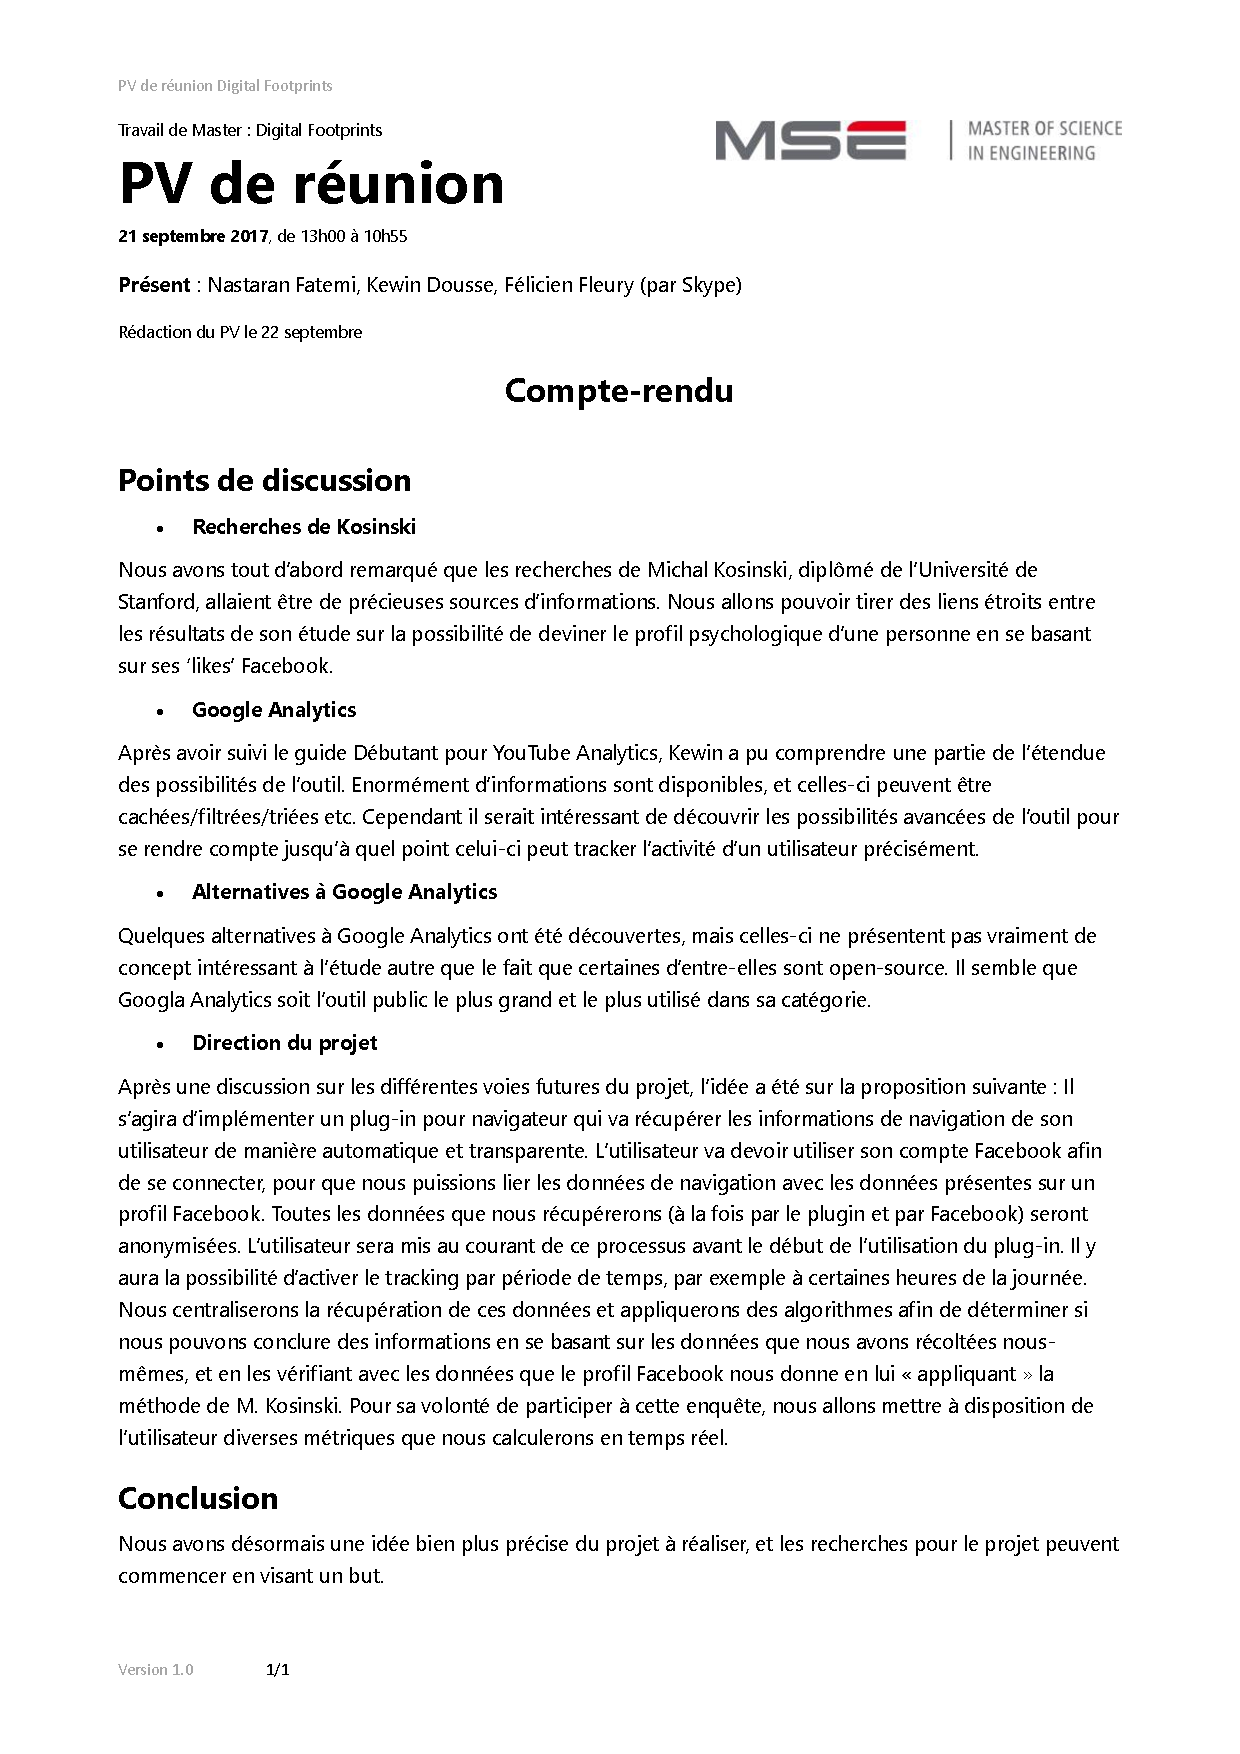
\includegraphics[width=1\textwidth]{images/annexes/pvs/DigFootprints_PV_21_09_2017}


\includegraphics[width=1\textwidth]{images/annexes/pvs/DigFootprints_PV_28_09_2017}

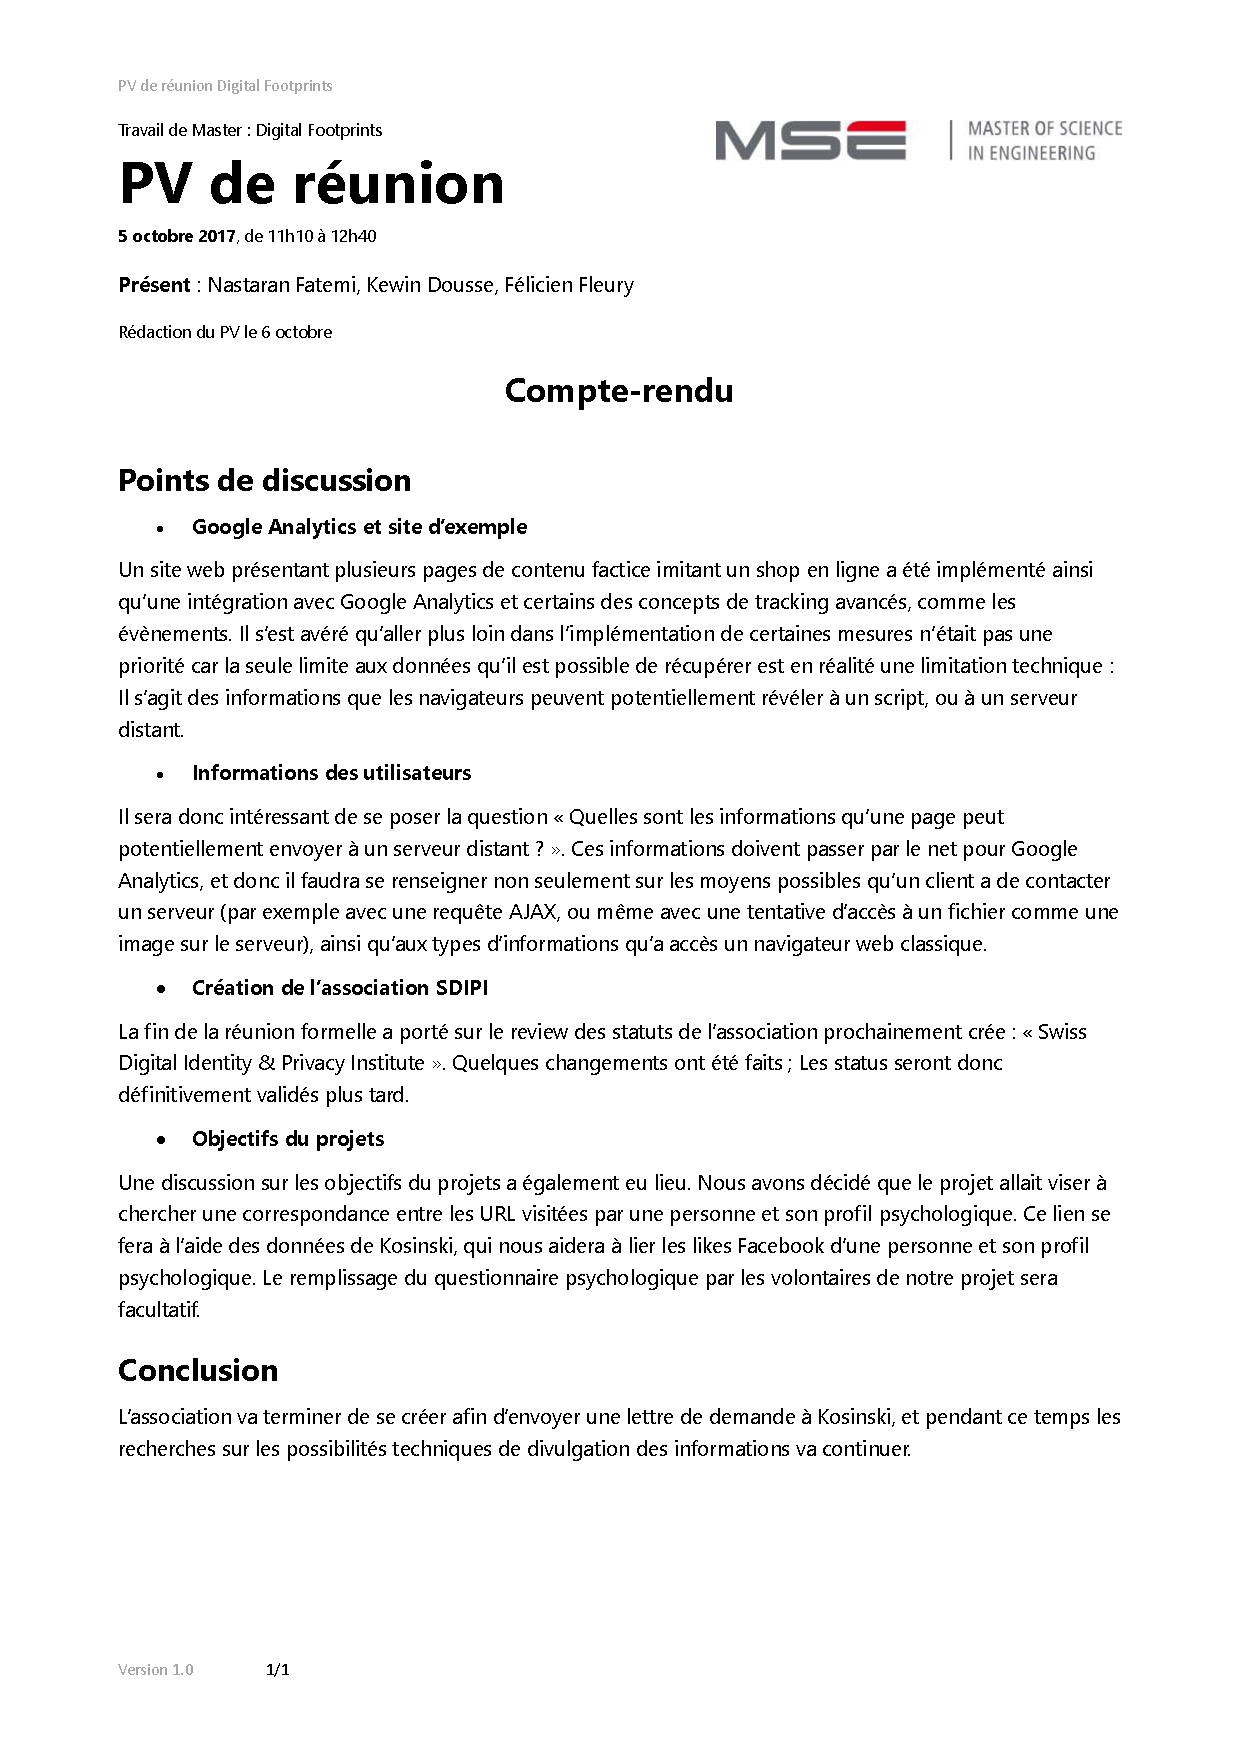
\includegraphics[width=1\textwidth]{images/annexes/pvs/DigFootprints_PV_05_10_2017}


\includegraphics[width=1\textwidth]{images/annexes/pvs/DigFootprints_PV_10_10_2017}


\includegraphics[width=1\textwidth]{images/annexes/pvs/DigFootprints_PV_12_10_2017}


\includegraphics[width=1\textwidth]{images/annexes/pvs/DigFootprints_PV_16_10_2017}


\includegraphics[width=1\textwidth]{images/annexes/pvs/DigFootprints_PV_26_10_2017}


\includegraphics[width=1\textwidth]{images/annexes/pvs/DigFootprints_PV_01_11_2017}


\includegraphics[width=1\textwidth]{images/annexes/pvs/DigFootprints_PV_09_11_2017}


\includegraphics[width=1\textwidth]{images/annexes/pvs/DigFootprints_PV_13_11_2017}


\includegraphics[width=1\textwidth]{images/annexes/pvs/DigFootprints_PV_16_11_2017}


\includegraphics[width=1\textwidth]{images/annexes/pvs/DigFootprints_PV_23_11_2017}


\includegraphics[width=1\textwidth]{images/annexes/pvs/DigFootprints_PV_30_11_2017}

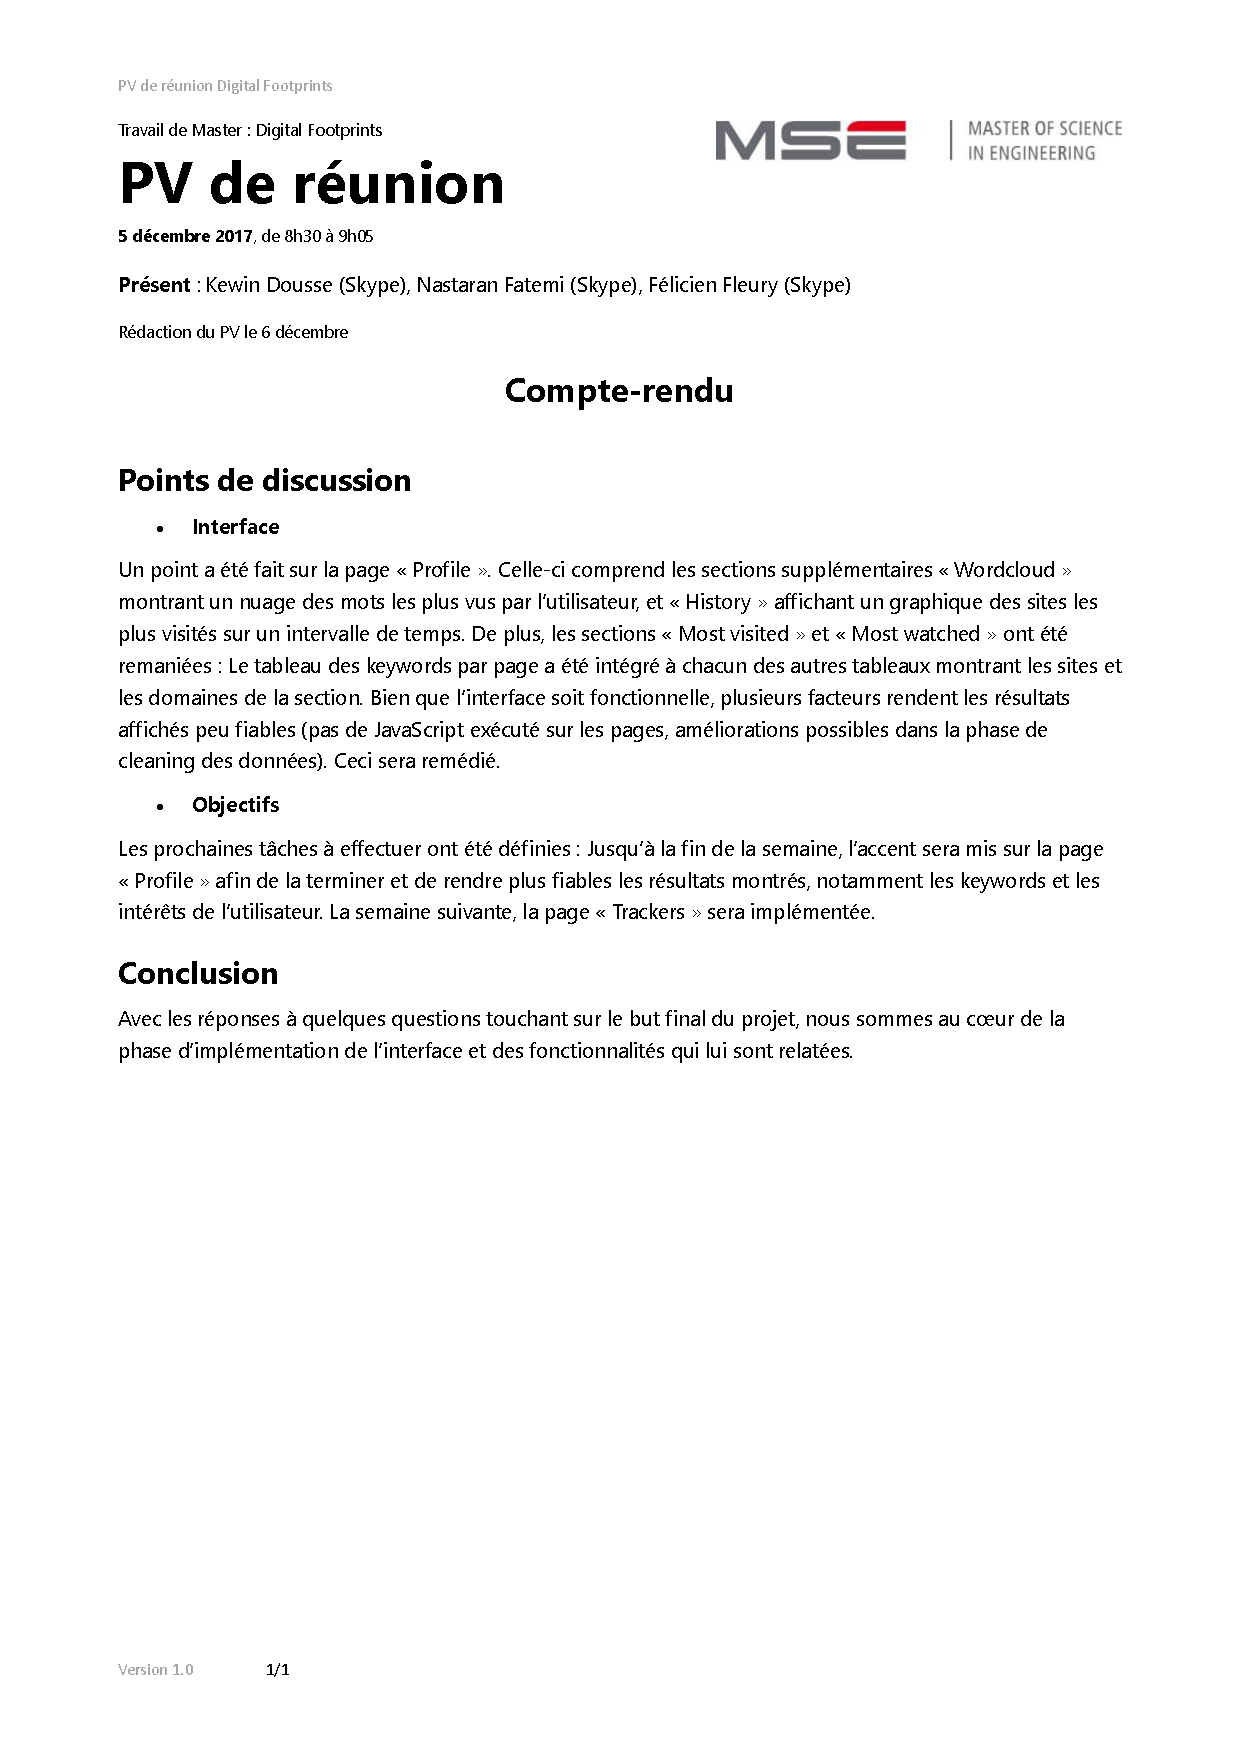
\includegraphics[width=1\textwidth]{images/annexes/pvs/DigFootprints_PV_05_12_2017}

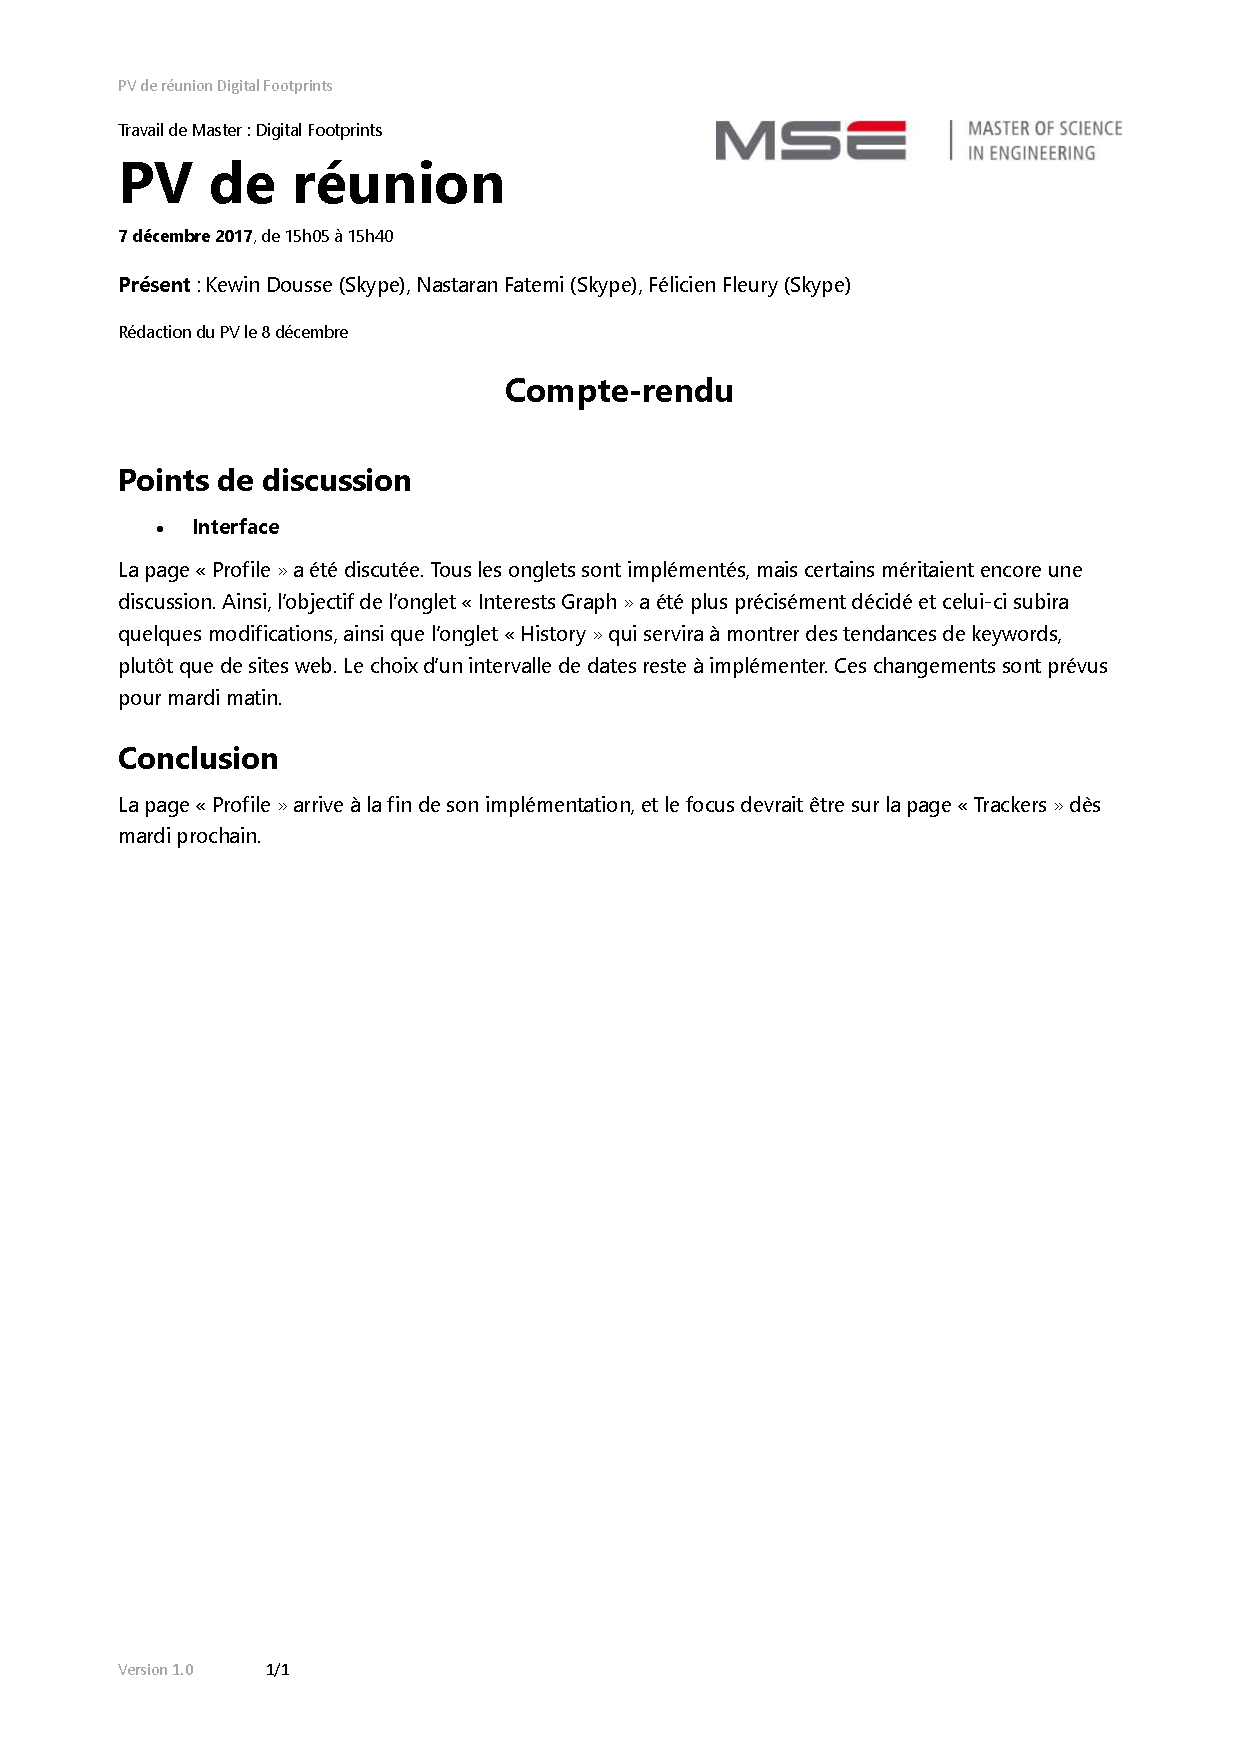
\includegraphics[width=1\textwidth]{images/annexes/pvs/DigFootprints_PV_07_12_2017}


\includegraphics[width=1\textwidth]{images/annexes/pvs/DigFootprints_PV_12_12_2017}

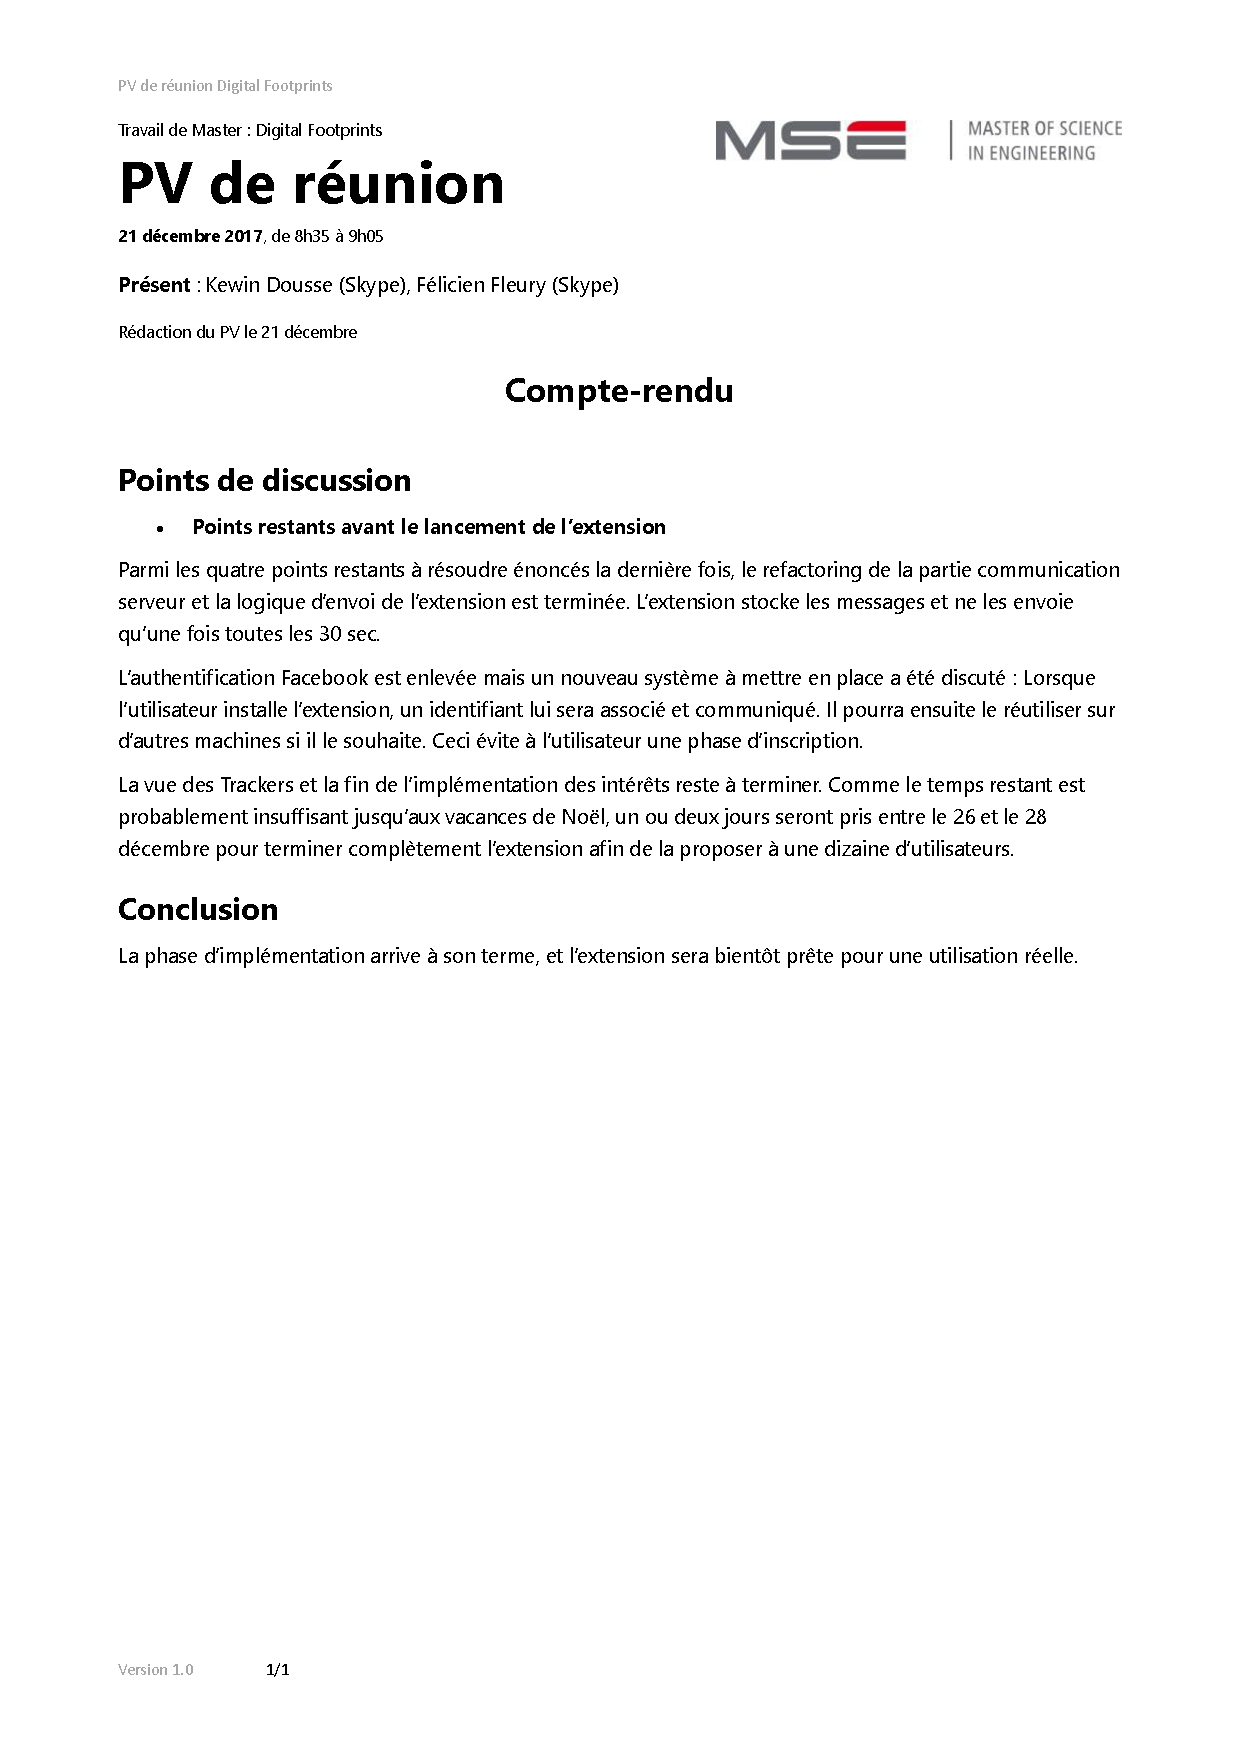
\includegraphics[width=1\textwidth]{images/annexes/pvs/DigFootprints_PV_21_12_2017}


\includegraphics[width=1\textwidth]{images/annexes/pvs/DigFootprints_PV_09_01_2018}


\includegraphics[width=1\textwidth]{images/annexes/pvs/DigFootprints_PV_18_01_2018}

\end{document}

% https://www.sharelatex.com/blog/2013/08/02/thesis-series-pt1.htmlx